\documentclass[12pt,a4paper]{article}
\usepackage[top=1in,bottom=1in,left=1.25in,right=1in]{geometry}
\usepackage{mathptmx}
\usepackage[T1]{fontenc}
\usepackage{xcolor}
\usepackage{array}
\usepackage{longtable}
\usepackage{colortbl}
\usepackage{enumitem}
\usepackage{setspace}
\usepackage{fancyhdr}
\usepackage{titlesec}
\usepackage[most]{tcolorbox}
\usepackage{microtype}
\usepackage{needspace}
\usepackage{graphicx}
\usepackage{float}
\usepackage{amsmath}
\usepackage{tikz}
\usetikzlibrary{positioning,arrows.meta,fit,backgrounds,calc,shapes.geometric}
\usepackage[hidelinks]{hyperref}
\usepackage{tocloft}
\usepackage{pgfplots}
\pgfplotsset{compat=1.16}
\renewcommand{\cftsecleader}{\cftdotfill{\cftdotsep}}
\setlength{\cftbeforesecskip}{3pt}

\definecolor{navy}{HTML}{000000}
\definecolor{purp}{HTML}{000000}
\definecolor{dred}{HTML}{000000}
\definecolor{azure}{HTML}{000000}
\definecolor{gbox}{HTML}{EAF2FA}
\definecolor{gborder}{HTML}{9AA5B1}
\definecolor{gtext}{HTML}{404040}
\definecolor{ghead}{HTML}{F2F2F2}
\definecolor{covergrey}{HTML}{767171}
\definecolor{tdark}{HTML}{3A3A3A}
\definecolor{tblue}{HTML}{1F3864}

\setstretch{1.4}
\setlength{\parindent}{0pt}
\setlength{\parskip}{6pt}
\pagestyle{empty}
\setlist{nosep}
\setlist[itemize]{leftmargin=2.2em,itemsep=2pt}

% Headings
\titleformat{\section}{\bfseries\fontsize{14}{17}\selectfont\color{purp}}{\thesection.}{0.3em}{}
\titleformat{\subsection}{\bfseries\large\color{navy}}{\thesubsection}{0.4em}{}
\titlespacing*{\section}{0pt}{14pt}{6pt}
\titlespacing*{\subsection}{0pt}{10pt}{4pt}
\newcommand{\redsec}[1]{\par\vspace{8pt}\addcontentsline{toc}{section}{#1}{\centering\bfseries\fontsize{14}{17}\selectfont #1\par}\vspace{2pt}\nopagebreak}
\newcommand{\purpsec}[1]{\par\vspace{8pt}\addcontentsline{toc}{section}{#1}{\centering\bfseries\fontsize{14}{17}\selectfont #1\par}\vspace{2pt}\nopagebreak}
\newcommand{\dredrule}{}
\newcommand{\bluesub}[1]{\par\vspace{4pt}\addcontentsline{toc}{subsection}{#1}{\bfseries #1\par}\nopagebreak}
\newcommand{\navysub}[1]{\par\vspace{4pt}\addcontentsline{toc}{subsection}{#1}{\bfseries #1\par}\nopagebreak}
\newcommand{\purpsub}[1]{\par\vspace{3pt}\addcontentsline{toc}{subsection}{#1}{\bfseries #1\par}\nopagebreak}

% Guideline box
\newtcolorbox{guide}[1]{enhanced,colback=gbox,colframe=gborder,boxrule=0.5pt,arc=0pt,
  left=6pt,right=6pt,top=3pt,bottom=3pt,
  fontupper=\itshape\small\color{gtext},before upper={\setstretch{1.15}\setlength{\parskip}{3pt}},
  title={\color{navy}\bfseries\upshape #1},coltitle=navy,colbacktitle=gbox,
  attach title to upper={\par},fonttitle=\small}

\setlength{\LTpre}{0pt}\setlength{\LTpost}{0pt}\setlength{\LTleft}{0pt}\setlength{\LTright}{0pt}

\begin{document}

% ---------------- COVER ----------------
\thispagestyle{empty}
\begin{tikzpicture}[remember picture,overlay]\draw[line width=2.5pt] ([shift={(1.5cm,1.5cm)}]current page.south west) rectangle ([shift={(-1.5cm,-1.5cm)}]current page.north east);\end{tikzpicture}
\begin{center}
\vspace*{0.6cm}
{\bfseries\fontsize{14}{17}\selectfont RV College of Engineering}\\[1.4cm]
{\itshape\color{gtext}\Large Experiential Learning (EL)}\\[0.5cm]
{\Large SDG 9 -- Industry, Innovation \& Infrastructure}\\[0.7cm]
\end{center}

\noindent\fbox{\parbox{\dimexpr\linewidth-2\fboxsep-2\fboxrule\relax}{\centering\vspace{6pt}
{\bfseries\LARGE PROJECT SYNOPSIS}\\[4pt]
{\small Phase 1}\vspace{8pt}}}\\[-1pt]
\renewcommand{\arraystretch}{1.75}
\setlength{\parskip}{0pt}
{\setlength{\fboxrule}{0.4pt}\noindent\hspace{-0pt}\begin{tabular}{|>{\raggedright\arraybackslash\bfseries\small}p{\dimexpr0.31\linewidth-12.4pt\relax}|p{\dimexpr0.69\linewidth-12.8pt\relax}|}
\hline
Title of Project: & {\hyphenpenalty=10000 \exhyphenpenalty=10000 AI-Driven Adaptive Physical Testing for Embedded Systems} \\ \cline{2-2}
Team No.: & 29 \\ \cline{2-2}
Student Name(s): & Kavin Krishnan C\newline Chinmai Kiran Shetti\newline Sumukha Upadhyaya\newline Snehal Reddy Thadigotla\newline Sutej R Haritsa \\ \cline{2-2}
USN / Reg. No.: & 1RV24CS126\newline 1RV24CS068\newline 1RV24IS130\newline 1RV24IS126\newline 1RV24CY055 \\ \cline{2-2}
Guide: & Dr. H K Krishnappa \\ \cline{2-2}
Semester: & Vth Semester \\ \cline{2-2}
Date of Submission: & 13 / 11 / 2026 \\ \hline
\end{tabular}}

\vspace{-0.2cm}
\begin{center}{\itshape\color{gtext}\small Academic Year: 2026--27}\end{center}

\newpage
\pagestyle{fancy}
\fancyhf{}
\fancyhead[L]{\raisebox{-0.25cm}{
\includegraphics[height=0.95cm]{figures/rvce-logo.png}}}
\fancyhead[R]{\small AI-Driven Adaptive Physical Testing for Embedded Systems}
\fancyfoot[C]{\small\thepage}
\renewcommand{\headrulewidth}{0.8pt}
\renewcommand{\footrulewidth}{0.8pt}
\setlength{\headheight}{30pt}
\addtolength{\topmargin}{-15.5pt}
\pagenumbering{roman}
\setcounter{tocdepth}{1}
\setstretch{1.15}
{\centering\bfseries\fontsize{14}{17}\selectfont Table of Contents\par}
\vspace{6pt}
{\setlength{\parskip}{0pt}\renewcommand{\contentsname}{}\makeatletter\@starttoc{toc}\makeatother}
\vspace{14pt}
{\centering\bfseries\fontsize{14}{17}\selectfont List of Abbreviations\par}
\vspace{6pt}
\renewcommand{\arraystretch}{1.25}
\begin{longtable}{|>{\raggedright\arraybackslash\bfseries}p{0.20\linewidth}|>{\raggedright\arraybackslash}p{0.70\linewidth}|}
\hline
AHFT & Adaptive Hardware Fuzzing Testbench \\ \hline
DUT & Device Under Test \\ \hline
HIL & Hardware-in-the-Loop \\ \hline
SDG & Sustainable Development Goal \\ \hline
MCU & Microcontroller Unit \\ \hline
ADC & Analog-to-Digital Converter \\ \hline
GPIO & General-Purpose Input/Output \\ \hline
LDR & Light-Dependent Resistor (photoresistor) \\ \hline
JSONL & JSON Lines (one JSON object per line) \\ \hline
REST / SSE & Representational State Transfer / Server-Sent Events \\ \hline
TPE & Tree-structured Parzen Estimator \\ \hline
GP-BO & Gaussian-Process Bayesian Optimisation \\ \hline
ET & ExtraTrees (extremely randomised trees) \\ \hline
PRD & Product Requirements Document \\ \hline
HLD & High-Level Design (document) \\ \hline
RQ & Research Question \\ \hline
\end{longtable}
\newpage
\pagenumbering{arabic}
\setcounter{page}{1}
\setstretch{1.4}

\purpsec{1. Abstract}
\dredrule
Embedded products fail under particular combinations of operating conditions such as supply voltage, workload, peripheral state and event timing. These combinations are rare among all possible ones, and testing every one of them on real hardware is too slow. Random testing wastes experiments in regions where the device already behaves correctly. This project builds a safety-constrained Adaptive Hardware Fuzzing Testbench (AHFT) that uses the results of earlier physical experiments to choose the next one.

An engineer writes a test contract that lists the controllable variables, measurable outputs, legal limits, hard safety limits and the failure requirement. A planner proposes a candidate experiment. A deterministic safety check accepts or rejects it in the backend and again in the bench controller. The controller applies the experiment to the device, collects synchronised measurements and returns the setup to a safe state. An independent oracle then labels the result.

The first deliverable targets timing failures on an ESP32. A laptop sends a six-parameter experiment (sampling interval, duration, sensor, task load, deadline and warm-up) over USB as JSON Lines. The board returns a microsecond timestamp record for every task release. The laptop recomputes every statistic from the raw samples and applies one frozen deadline rule, so the firmware's own summary is only advisory. Adaptive selection uses an ExtraTrees surrogate whose acquisition combines failure probability, model uncertainty and novelty, and it is compared with random, grid, TPE and space-filling baselines at equal experiment budgets. Failures are confirmed and minimised. The software is built simulator-first, with disclosed seeded timing defects, so that connecting the real board changes one adapter. The expected outcome is a reproducible testbench and honest evidence on whether adaptive search finds failures in fewer physical experiments, without treating the absence of a failure as proof of safety.

\textbf{Keywords:} {\itshape Adaptive Testing, Hardware-in-the-Loop, Embedded Systems, Timing Failures, Fuzzing, Surrogate Models, ExtraTrees, Safety-Constrained Search, ESP32}

\newpage
\purpsec{2. Introduction}

\navysub{2.1 Background}
This project is aligned with UN Sustainable Development Goal 9 (Industry, Innovation and Infrastructure), Target 9.5, which supports technological research and the upgrading of industrial technologies~[1]. Cheaper and more systematic validation of embedded hardware is a concrete step toward it.

Embedded systems sit inside cars, medical devices, factory equipment and consumer electronics, and the cost of a field failure is high. Their failures are often not caused by one wrong input. They appear when several conditions coincide: a supply rail near its lower limit while the processor is busy and a peripheral is mid-transfer, or a short sampling period combined with heavy computation. A firmware build that looks correct at nominal settings can still miss deadlines, drift in timing or reset under such a combination.

Software testing has a mature answer to a large input space. Fuzzers keep inputs that reach new behaviour and mutate them, instead of enumerating everything~[2]. Surveys of embedded fuzzing show that the idea has been carried to firmware, but also that crash detection is harder on embedded targets and that tools are hard to compare~[3],[4]. Most of that work stays in emulation or on the bytes delivered to the firmware. It does not vary the electrical and timing conditions of a real device, which is where many embedded faults live.

Hardware experiments are also expensive. One physical run takes seconds to minutes, has measurement noise, and can wear or stress equipment. A search for failures therefore has to spend a small budget of experiments well and must never leave the limits that keep the board and the bench safe.

\navysub{2.2 Problem Statement}
Conventional embedded testing either sweeps a grid or samples at random, and neither learns from the experiments already run. Adaptive search methods exist, but they are mostly demonstrated in simulation or in software, and they do not combine a reviewed safety envelope, trustworthy physical measurement and failure minimisation in one test loop. There is no small, reproducible testbench that lets a team ask whether feedback-driven selection finds embedded failures in fewer physical experiments than conventional selection, without running anything outside the permitted limits.

\navysub{2.3 Motivation}
A team that spends its budget on settings that are known to pass learns nothing, and a team that spends it beyond the limits may damage the device. A testbench that chooses informative experiments, refuses unsafe ones in two independent places, and stores enough evidence to replay and shrink every failure would make validation faster and safer. A reproducible open design also lets others test planning methods on real hardware under identical rules, which supports the research and innovation aims of SDG~9.

\redsec{3. Literature Survey / Review of Related Work}
\dredrule

\navysub{3.1 Fuzzing and Firmware Testing}
American Fuzzy Lop popularised a feedback loop that keeps inputs producing new behaviour and mutates promising seeds rather than relying on blind generation~[2]. The transferable idea is feedback-guided allocation of test effort. Yun et al.~[3] survey fuzzing of embedded and IoT firmware, covering emulation, multi-architecture support and why crash detection is harder in embedded targets, and Eisele et al.~[4] classify embedded fuzzers by how they interface with the target and note the lack of standard cross-tool benchmarks. Rehosting tools replace hardware abstraction layers (HALucinator~[5]), model peripheral interfaces automatically (P$^2$IM~[6]) or model memory-mapped input/output precisely (Fuzzware~[7]) to fuzz firmware in an emulator. $\mu$AFL~[8] connects a host fuzzer to a real microcontroller and uses processor trace features for feedback, and E-FuzzEdge~[9] reduces communication overhead in in-place fuzzing. These systems fuzz the bytes that reach the firmware. None of them varies the electrical conditions or workload timing of the device, and emulation cannot reproduce power integrity, component tolerance or unit-to-unit variation.

\navysub{3.2 Combinatorial and Space-Filling Test Design}
Combinatorial testing covers all chosen low-order interactions of discrete values with far fewer tests than an exhaustive sweep~[10]. It is a strong baseline for categorical states, but it is not adaptive and needs discretisation, so it can miss a narrow failing region between two chosen levels of a continuous variable. Latin hypercube sampling stratifies each variable's range and gives broad initial coverage~[11]. In this project both are used as baselines or warm starts, not as the contribution.

\navysub{3.3 Active Learning and Safe Optimisation}
Bryan et al.~[12] select experiments to locate function threshold boundaries with entropy and variance criteria, and Gotovos et al.~[13] estimate level sets with Gaussian processes and confidence-bound sampling. They motivate the goal of learning a pass/fail boundary from few samples. SafeOpt~[14] explores an unknown function while staying above a safety threshold under a Gaussian-process assumption, and Berkenkamp et al.~[15] extend it to several safety constraints and apply it to robot parameter tuning. Their assumptions matter: a physical response surface can be discontinuous, stochastic and categorical, and a smooth model can be confidently wrong. In this project the learned model only guides the choice among candidates. The hard limits are checked by deterministic rules that the model cannot override.

\navysub{3.4 Falsification, Hardware-in-the-Loop and Adaptive Fault Injection}
Temporal-logic falsification tools search for inputs that give the lowest robustness value for a requirement, and a negative robustness is a counterexample~[16]. Adaptive stress testing frames rare-failure discovery as a sequential search~[17]. Hardware-in-the-loop testing is established engineering: PHiLIP offers an external reference device for automated multi-platform embedded-OS testing~[18], and IEEE 2004-2025 gives a recommended practice for HIL simulation-based testing~[19]. The closest recent precedent is GlitchLab, an unreviewed preprint that adaptively optimises physical voltage and timing fault injection for security faults~[20]. It deliberately perturbs execution beyond normal operation, whereas this project stays inside the product's approved non-destructive envelope and targets product requirements.

\navysub{3.5 Surrogate Models, Minimisation and Benchmarking}
The Tree-structured Parzen Estimator models good and bad configurations with two densities and proposes points that maximise their ratio~[21]. Extremely randomised trees build an ensemble with random split features and thresholds, which is cheap to train on small data sets, and the spread of the trees gives a heuristic uncertainty~[22]. The Optuna framework provides TPE and the random samplers used here as adaptive and baseline planners~[23]. Delta debugging simplifies a failure-inducing input to a minimal one~[24]; this project applies the same idea to physical experiments. FuzzBench argues that fuzzer claims need repeated trials, shared benchmarks and raw data~[25], which this project adopts as a requirement.

\navysub{3.6 Research Gap Summary}
\par\nopagebreak\noindent{\setstretch{1}\small\bfseries Table 3.1: Research gap summary}\par\nopagebreak\vspace{2pt}
\renewcommand{\arraystretch}{1.5}
\begin{longtable}{|>{\raggedright\arraybackslash\setlength{\parskip}{0pt}\setstretch{1}}p{0.17\linewidth}|>{\raggedright\arraybackslash\setlength{\parskip}{0pt}\setstretch{1}}p{0.27\linewidth}|>{\raggedright\arraybackslash\setlength{\parskip}{0pt}\setstretch{1}}p{0.46\linewidth}|}
\hline
\rowcolor{ghead}\bfseries Reference & \bfseries Key Contribution & \bfseries Limitation / Research Gap \\ \hline
Yun et al., 2023 [3]; Eisele et al., 2022 [4] & Surveys of embedded and IoT fuzzing & Taxonomy only; no standard benchmark and no search over electrical or timing conditions \\ \hline
Clements et al., 2020 [5]; Feng et al., 2020 [6]; Scharnowski et al., 2022 [7] & Firmware rehosting and peripheral modelling for emulated fuzzing & Emulation cannot reproduce power integrity, tolerances or unit variation \\ \hline
Li et al., 2022 [8]; Rusconi et al., 2026 [9] & Feedback fuzzing of real microcontrollers & Input is bytes delivered to firmware; external conditions are not varied \\ \hline
Kuhn et al., 2010 [10] & Combinatorial covering arrays & Not adaptive; needs discretisation of continuous variables \\ \hline
Sui et al., 2015 [14]; Berkenkamp et al., 2023 [15] & Safe exploration with Gaussian processes & Smooth-model assumptions; demonstrated on robots and simulation, not a reviewed embedded test bench \\ \hline
Annapureddy et al., 2011 [16] & Temporal-logic falsification & Needs a simulator model; no electrical safety enforcement or instrument uncertainty \\ \hline
Hossain et al., 2026 [20] (preprint) & Adaptive HIL fault injection & Security-oriented glitching outside the normal envelope; not product requirements \\ \hline
Zeller and Hildebrandt, 2002 [24] & Delta debugging & Defined for software inputs, not stochastic physical episodes \\ \hline
\end{longtable}

\redsec{4. Objectives}
\dredrule
The primary objectives of this project are:
\begin{itemize}
\item To design a safety-constrained test loop in which an engineer-written contract, a planner, a backend safety check, a bench controller and an oracle each have one clear job, and in which no experiment outside the declared limits is executed.
\item To build a bench that executes physical experiments on an ESP32 over a typed JSON-Lines protocol and records microsecond-resolution raw samples, with every summary statistic recomputed independently on the PC.
\item To implement an adaptive planner (ExtraTrees surrogate with a failure-probability, uncertainty and novelty acquisition) and compare it with random, grid, TPE and space-filling selection at equal experiment budgets.
\item To confirm each discovered failure, reduce it to a minimal set of conditions, and publish the exact experiment sequence, raw traces and safety decisions so that every result can be replayed.
\end{itemize}

\navysub{4.1 Scope and Delimitations}
\begin{itemize}
\item\relax \emph{In scope for version 1 (Feature 1):} timing-failure detection on an ESP32 using a software-defined synthetic workload, an LDR or potentiometer as the sensor under test, a deterministic simulator with disclosed seeded defects, and a seven-view operator dashboard.
\item\relax \emph{In scope for the wider platform:} the test contract, two-layer safety check, controller and console, and the multi-rail OLED demonstration (programmable supply rails, an ESP32-S3 device and a test-controller MCU) that carries the safety design.
\item\relax \emph{Out of scope:} destructive or security fault injection, Wi-Fi and Bluetooth workloads, multiple devices, unattended operation, worst-case-execution-time guarantees, and any claim that a device is proven safe.
\end{itemize}

\redsec{5. Proposed Methodology}
\dredrule

\bluesub{5.1 System Architecture Overview}
The system is split into a control plane on the laptop and a bench plane beside the physical hardware (Figure 5.1). The researcher works in a web console, written in Next.js, whose server routes add the operator token so that the browser never holds it. The backend owns the test contract, the campaign state and the first safety check, and it keeps an append-only audit log in a relational database (SQLite in version 1). The Agent service manages the campaign lifecycle and the experiment budget and asks the Decision service for the next candidate. The Oracle judges measured behaviour. On the bench plane, the Controller claims an approved experiment, re-checks the limits against the live bench state, applies the conditions through the Adapter, collects measurements and returns the setup to a safe state. The Adapter hides the instrument: in simulation it is a deterministic simulated ESP32, and on hardware it is a serial link, so switching is a device-configuration change and not a code change. The Backend and the Controller share one safety-rule library. All application services are written in Python.

\begin{figure}[t]
\centering
\resizebox{\linewidth}{!}{%
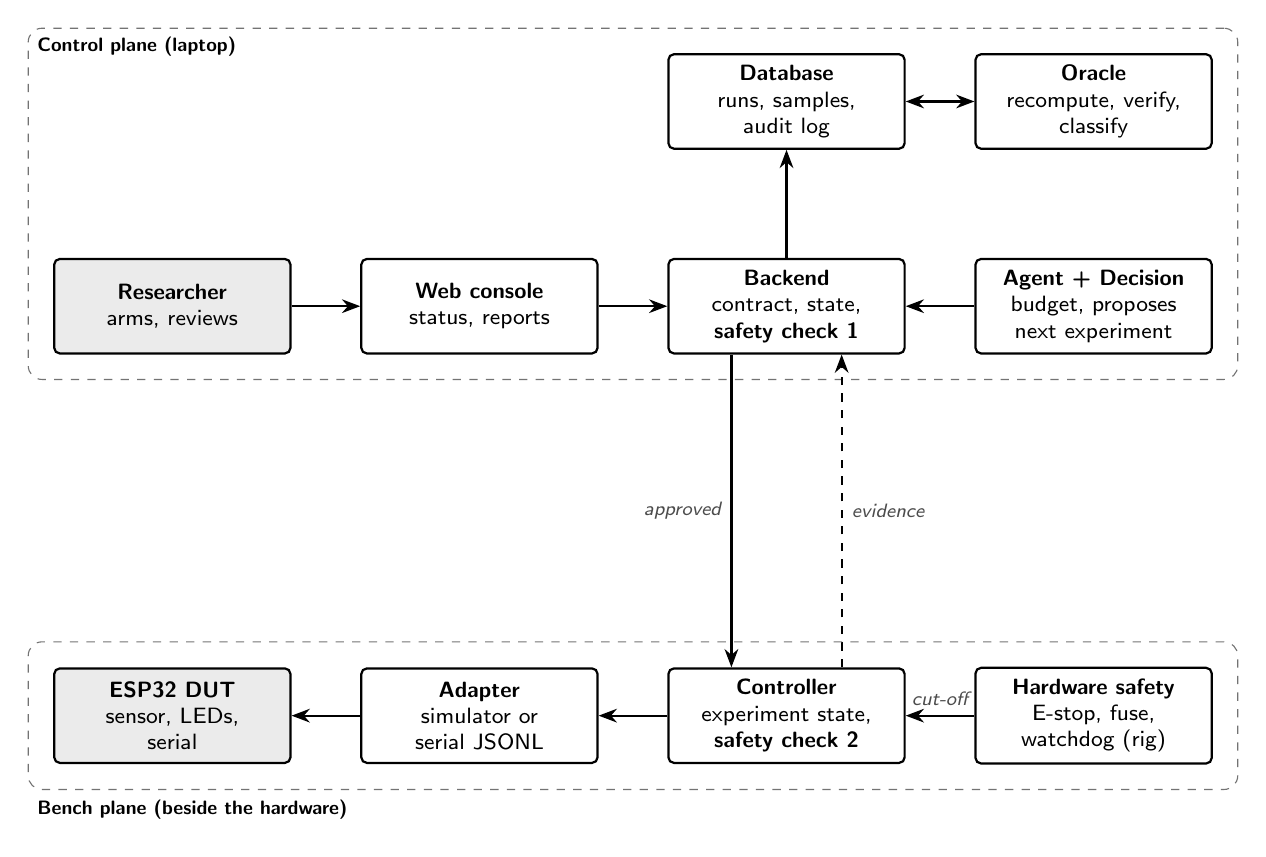
\begin{tikzpicture}[
  font=\sffamily\footnotesize,
  >=Stealth,
  box/.style={draw=black,rounded corners=2pt,thick,align=center,inner sep=4pt,fill=white,minimum height=1.2cm,minimum width=3.0cm},
  io/.style={box,fill=black!8},
  grp/.style={draw=black!55,dashed,rounded corners=5pt,inner sep=9pt},
  lbl/.style={font=\sffamily\scriptsize\itshape,black!70},
  arr/.style={->,thick}
]
\node[io] (res) at (0,0) {\textbf{Researcher}\\arms, reviews};
\node[box] (con) at (3.9,0) {\textbf{Web console}\\status, reports};
\node[box] (back) at (7.8,0) {\textbf{Backend}\\contract, state,\\\textbf{safety check 1}};
\node[box] (plan) at (11.7,0) {\textbf{Agent + Decision}\\budget, proposes\\next experiment};
\node[box] (db) at (7.8,2.6) {\textbf{Database}\\runs, samples,\\audit log};
\node[box] (orc) at (11.7,2.6) {\textbf{Oracle}\\recompute, verify,\\classify};
\draw[arr] (res) -- (con);
\draw[arr] (con) -- (back);
\draw[arr] (plan) -- (back);
\draw[arr] (back) -- (db);
\draw[arr,<->] (db) -- (orc);
\node[grp,fit=(res)(con)(back)(plan)(db)(orc),label={[font=\sffamily\scriptsize\bfseries,anchor=north west]north west:Control plane (laptop)}] (cp) {};
\node[io] (dut) at (0,-5.2) {\textbf{ESP32 DUT}\\sensor, LEDs,\\serial};
\node[box] (ada) at (3.9,-5.2) {\textbf{Adapter}\\simulator or\\serial JSONL};
\node[box] (ctl) at (7.8,-5.2) {\textbf{Controller}\\experiment state,\\\textbf{safety check 2}};
\node[box] (safe) at (11.7,-5.2) {\textbf{Hardware safety}\\E-stop, fuse,\\watchdog (rig)};
\draw[arr] ([xshift=-0.7cm]back.south) -- node[left,lbl,pos=0.5]{approved} ([xshift=-0.7cm]ctl.north);
\draw[arr,dashed] ([xshift=0.7cm]ctl.north) -- node[right,lbl,pos=0.5]{evidence} ([xshift=0.7cm]back.south);
\draw[arr] (ctl) -- (ada);
\draw[arr] (ada) -- (dut);
\draw[arr] (safe) -- node[above,lbl]{cut-off} (ctl);
\node[grp,fit=(dut)(ada)(ctl)(safe),label={[font=\sffamily\scriptsize\bfseries,anchor=north west]south west:Bench plane (beside the hardware)}] (bp) {};
\end{tikzpicture}}\\[4pt]
{\setstretch{1}\small\itshape Figure 5.1: Proposed system architecture (control plane and bench plane).}
\end{figure}

Safety is layered so that no single component is trusted alone: the backend checks every candidate against the contract limits, the controller re-checks against the live bench before running, the instruments enforce their own limits, and a watchdog, fuse and E-stop on the multi-rail rig cut power independently of software. A candidate that fails any check is rejected with structured reasons, is never clamped to a nearby legal value, is never executed and is never used for training. The practice follows the principle that hazards in laboratory electrical equipment are controlled by design and not by procedure~[26].

\bluesub{5.2 Test Bench Hardware}
Version 1 uses an ESP32-WROOM-32 DevKit~[26] on a breadboard, connected to the laptop by a micro-USB cable (Figure 5.2). A photoresistor (LDR) is wired to GPIO34 and a trimmer potentiometer to GPIO35, both read by the 12-bit ADC (raw range 0--4095); a third channel, \texttt{ADC\_SIM}, is synthetic. Figure 5.3 shows a typical 30-pin DevKit of this kind: the module with its PCB antenna under a metal shield, a USB-to-UART bridge (a CP2102 in the model), a 3.3\,V regulator (AMS1117), EN and BOOT buttons and a power and a GPIO2 LED. The parts on the physical board will be confirmed by the hardware team. The device runs a synthetic workload whose size, \texttt{task\_load}, is expressed in calibrated work units so that the load is repeatable across boards. Version 1 changes no voltages and drives no external loads, so it adds no electrical hazard beyond USB-powered bench work. The exact module (WROOM-32 or S3) is to be confirmed by the hardware team and the device reports it truthfully in its capability reply. The multi-rail platform for the OLED demonstration (an ESP32-S3 device, an RP2040 test controller and three programmable extra-low-voltage rails) remains the long-term rig.

\begin{figure}[t]
\centering
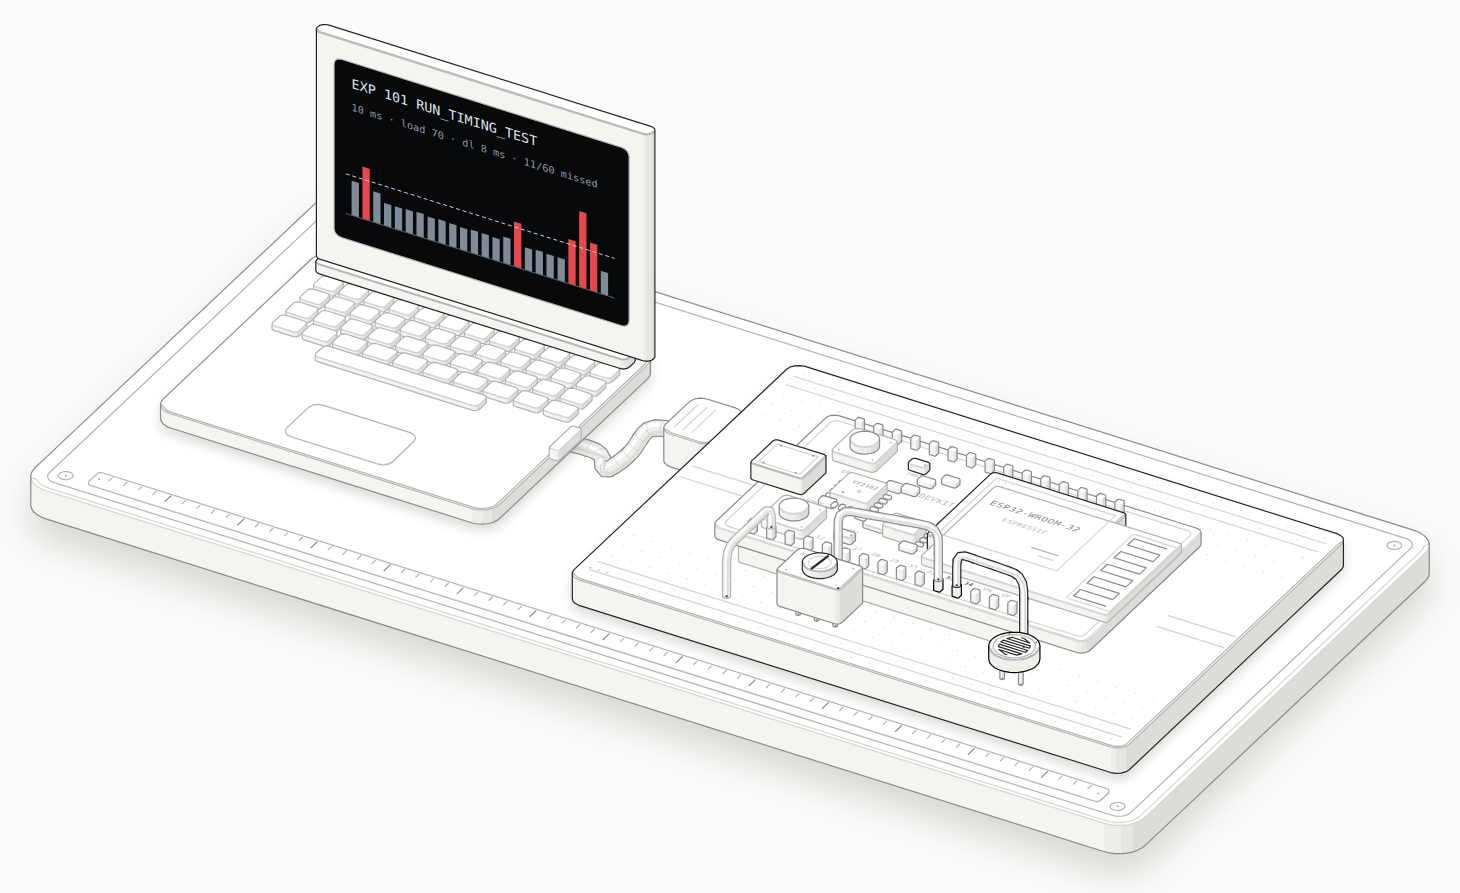
\includegraphics[width=\linewidth]{figures/anatomy/crop-fig1-bench.png}\\[2pt]
{\setstretch{1}\small\itshape Figure 5.2: The timing bench (isometric model built from the project's bench design). The laptop screen shows, for each task release, how long after its scheduled time the task finished relative to its deadline (dashed line); missed deadlines are the dark bars. The bars come from the same timing model as the project simulator (seeded defect A shown), not from a physical board.}
\end{figure}

\begin{figure}[t]
\centering
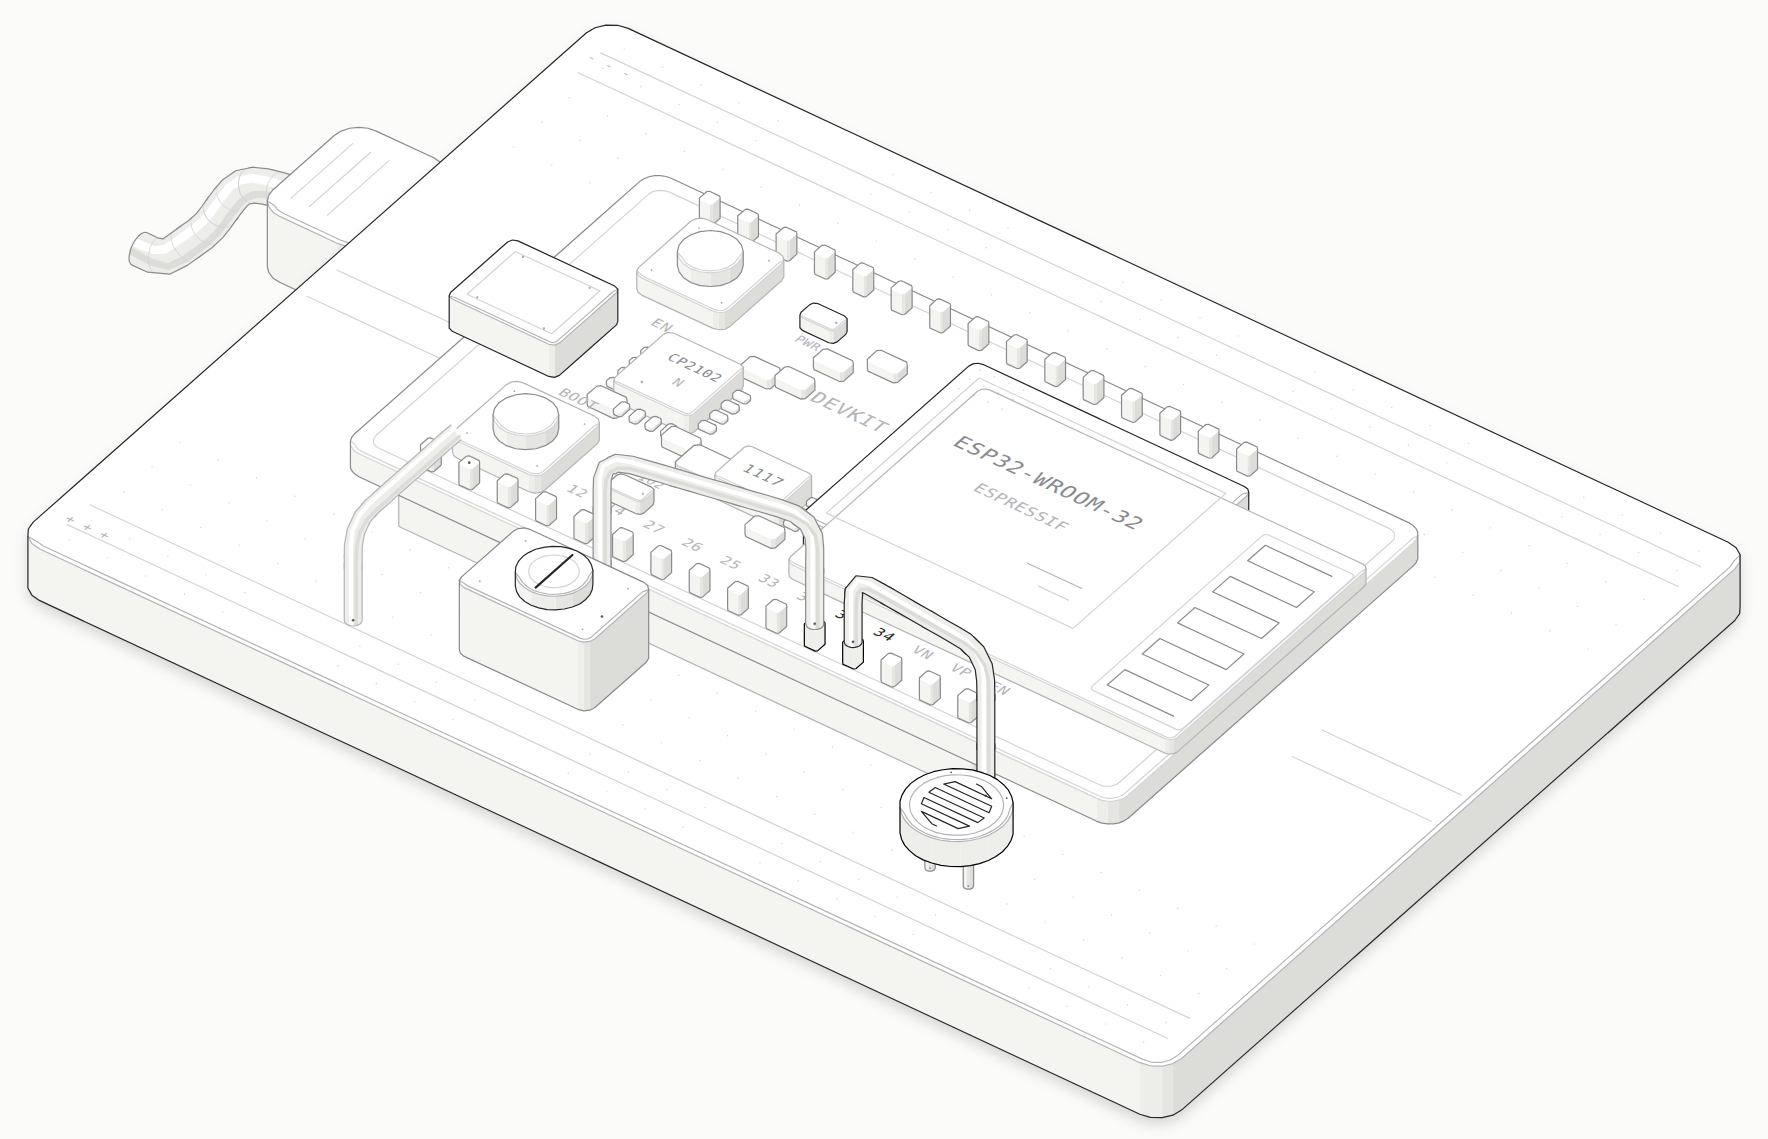
\includegraphics[width=0.96\linewidth]{figures/anatomy/crop-fig2-devkit.png}\\[2pt]
{\setstretch{1}\small\itshape Figure 5.3: Model of a typical ESP32-WROOM-32 DevKit on the breadboard: shielded module with PCB antenna, CP2102 bridge, AMS1117 regulator, EN and BOOT buttons, header pins (GPIO34 and GPIO35 emphasised) and the micro-USB plug. The 3.3\,V feed and the pull-down resistor are omitted for clarity.}
\end{figure}

\bluesub{5.3 Experiment Description and Data}
The data of this project are experiment records produced by the bench, not a pre-collected data set. An experiment is a six-variable configuration sent from the PC to the ESP32 as one UTF-8 JSON line. The device answers with an acknowledgement, one raw sample frame per scheduled task release and a final summary. Every frame carries a protocol version, and a mismatch is rejected. The capability envelope below is reported by the device and is enforced on both the PC and the device.

\par\nopagebreak\noindent{\setstretch{1}\small\bfseries Table 5.1: Experiment input variables and capability envelope}\par\nopagebreak\vspace{2pt}
\renewcommand{\arraystretch}{1.4}
\begin{longtable}{|>{\raggedright\arraybackslash\setlength{\parskip}{0pt}\setstretch{1}\small\ttfamily}p{0.27\linewidth}|>{\raggedright\arraybackslash\setlength{\parskip}{0pt}\setstretch{1}\small}p{0.16\linewidth}|>{\raggedright\arraybackslash\setlength{\parskip}{0pt}\setstretch{1}\small}p{0.45\linewidth}|}
\hline
\rowcolor{ghead}\bfseries\rmfamily Variable & \bfseries\rmfamily Range & \bfseries\rmfamily Meaning \\ \hline
sampling\_interval\_ms & 5--1000 ms & Period between scheduled task releases \\ \hline
duration\_ms & 100--30000 ms & Length of the measured window \\ \hline
sensor\_type & LDR, POT, ADC\_SIM & Sensor channel read in each task \\ \hline
task\_load & 0--100 units & Calibrated synthetic work per release \\ \hline
deadline\_ms & 2--1000 ms & Relative deadline from each scheduled release \\ \hline
warmup\_ms & 0--5000 ms & Initial window excluded from all statistics \\ \hline
\end{longtable}

Integers only are accepted for integer fields (no booleans, floats or strings). All problems of a bad request are returned together with codes such as \texttt{MISSING\_FIELD}, \texttt{INVALID\_TYPE}, \texttt{OUT\_OF\_RANGE}, \texttt{UNSUPPORTED\_SENSOR} and \texttt{INVALID\_WINDOW}, and the device buffer limit of 4096 samples per experiment is a derived constraint. For each release the device records, from one monotonic microsecond clock, the scheduled time, the actual start time, the execution time, the sensor value, a read-success flag, an error code, the boot identifier and a warm-up flag. The PC derives start lateness, completion time and inter-sample interval from these and never trusts the firmware for them. The deadline rule is frozen:
\begin{center}
a sample misses its deadline if and only if\quad $t_{\text{actual}} + t_{\text{exec}} > t_{\text{scheduled}} + 1000\cdot d_{\text{ms}}$.
\end{center}
Both start lateness and execution time therefore count, because the deadline is anchored at the scheduled release. Jitter is the sample standard deviation of the inter-sample intervals, and the deadline miss rate is the number of misses divided by the number of scheduled samples, so samples that never arrived still count against the device.

\bluesub{5.4 Proposed Algorithm / Model}
The episode loop (Figure 5.4) is the same for every strategy, so that strategies differ only in how they pick the next experiment.

\begin{figure}[t]
\centering
\resizebox{\linewidth}{!}{%
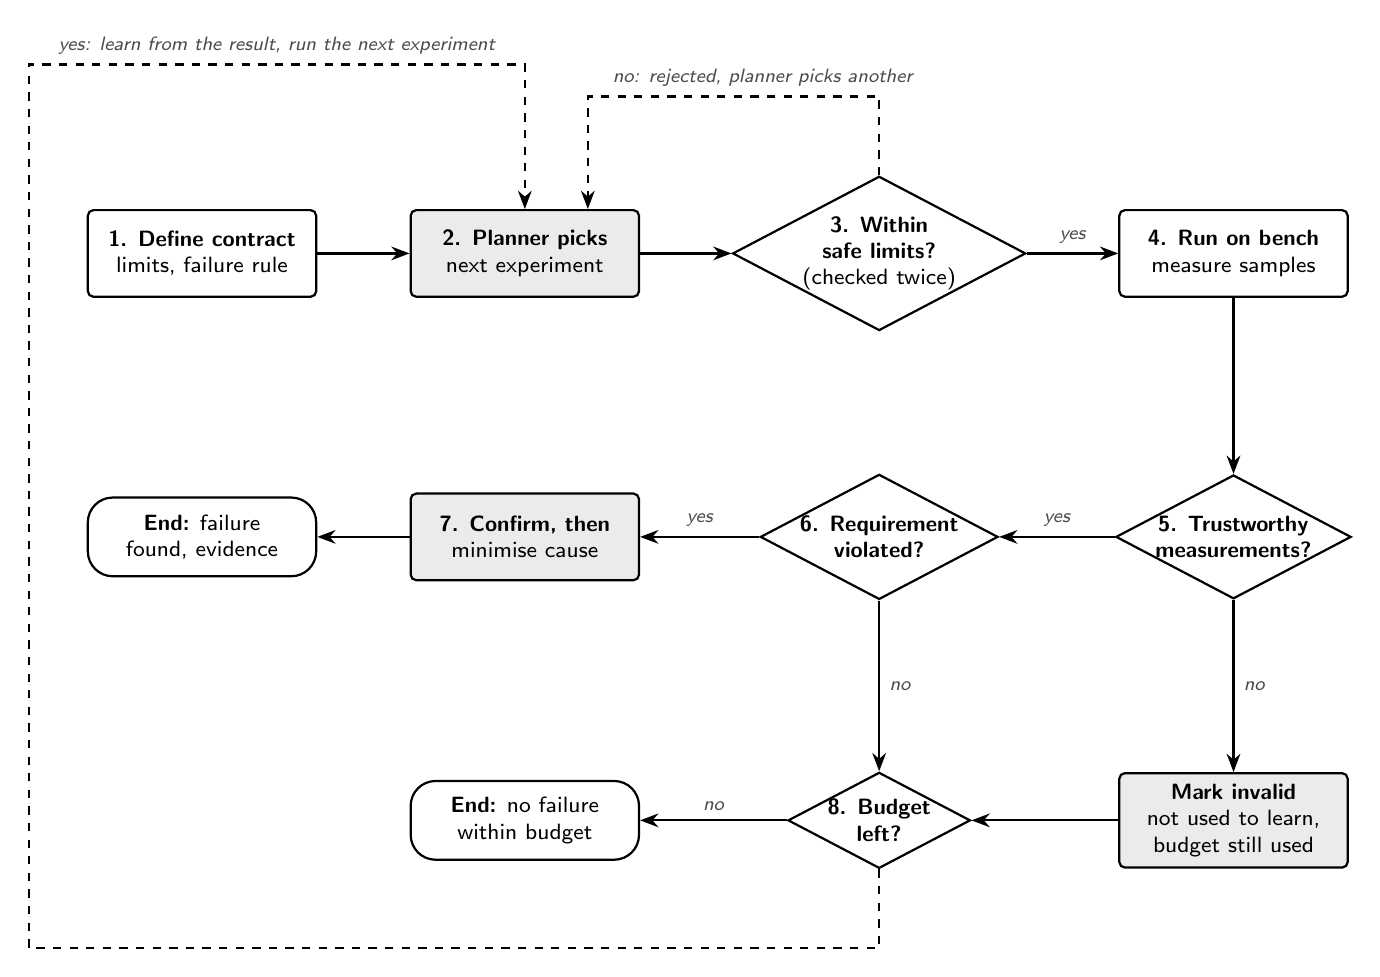
\begin{tikzpicture}[
  font=\sffamily\footnotesize,
  >=Stealth,
  box/.style={draw=black,rounded corners=2pt,thick,align=center,inner sep=4pt,fill=white,minimum height=1.1cm,minimum width=2.9cm},
  pl/.style={box,fill=black!8},
  dec/.style={draw=black,diamond,aspect=1.9,thick,align=center,inner sep=0pt,fill=white},
  term/.style={draw=black,rounded corners=9pt,thick,align=center,inner sep=4pt,minimum height=1.0cm,minimum width=2.9cm,fill=white},
  lbl/.style={font=\sffamily\scriptsize\itshape,black!70},
  arr/.style={->,thick}
]
\node[box] (ctr) at (0,0) {\textbf{1. Define contract}\\limits, failure rule};
\node[pl] (pln) at (4.1,0) {\textbf{2. Planner picks}\\next experiment};
\node[dec] (saf) at (8.6,0) {\textbf{3. Within}\\\textbf{safe limits?}\\(checked twice)};
\node[box] (run) at (13.1,0) {\textbf{4. Run on bench}\\measure samples};
\node[dec] (trs) at (13.1,-3.6) {\textbf{5. Trustworthy}\\\textbf{measurements?}};
\node[dec] (vio) at (8.6,-3.6) {\textbf{6. Requirement}\\\textbf{violated?}};
\node[pl] (cmf) at (4.1,-3.6) {\textbf{7. Confirm, then}\\minimise cause};
\node[term] (fnd) at (0,-3.6) {\textbf{End:} failure\\found, evidence};
\node[box,fill=black!8] (inv) at (13.1,-7.2) {\textbf{Mark invalid}\\not used to learn,\\budget still used};
\node[dec] (bud) at (8.6,-7.2) {\textbf{8. Budget}\\\textbf{left?}};
\node[term] (nof) at (4.1,-7.2) {\textbf{End:} no failure\\within budget};
\draw[arr] (ctr) -- (pln);
\draw[arr] (pln) -- (saf);
\draw[arr] (saf) -- node[above,lbl]{yes} (run);
\draw[arr] (run) -- (trs);
\draw[arr] (trs) -- node[above,lbl]{yes} (vio);
\draw[arr] (vio) -- node[above,lbl]{yes} (cmf);
\draw[arr] (cmf) -- (fnd);
\draw[arr] (trs) -- node[right,lbl]{no} (inv);
\draw[arr] (inv) -- (bud);
\draw[arr] (vio) -- node[right,lbl]{no} (bud);
\draw[arr] (bud) -- node[above,lbl]{no} (nof);
\draw[arr,dashed] (saf.north) -- ++(0,1.0) -| node[above,lbl,pos=0.2]{no: rejected, planner picks another} ([xshift=0.8cm]pln.north);
\draw[arr,dashed] (bud.south) -- ++(0,-1.0) -| (-2.2,-8.2) -- (-2.2,2.4) -- node[above,lbl,pos=0.5]{yes: learn from the result, run the next experiment} (4.1,2.4) -- (pln.north);
\end{tikzpicture}}\\[4pt]
{\setstretch{1}\small\itshape Figure 5.4: The adaptive experiment loop with two safety checks, a trust check on the measurements, confirmation and minimisation.}
\end{figure}

\textbf{Step 1: warm start.} Until four labelled experiments exist, the planner draws safe candidates that maximise their distance from experiments already run, so that the surrogate is never fitted on a handful of points.

\textbf{Step 2: surrogate.} The planner fits an ensemble of 25 extremely randomised trees~[22] on earlier experiments of the same campaign. The inputs are only the six pre-execution variables, never jitter, miss rate, outcome or signature, and the label is the oracle's failure label. A passing experiment that came close to its deadline carries a failure-proximity target between 0 and 0.85, so near-limit passes still inform the model. The mean of the trees is the failure probability $\hat P(x)$, and their standard deviation $\hat U(x)$ is a heuristic uncertainty.

\textbf{Step 3: acquisition.} Each candidate in a pool of unseen, safe configurations is scored by
\begin{equation*}
A(x) = \alpha\,\hat P(\text{fail}\mid x) + \beta\,\hat U(x) + \gamma\,\widehat{\text{Novelty}}(x),
\end{equation*}
where Novelty is the distance to the nearest experiment already run, each term is min--max normalised over the pool, and the defaults are $\alpha=0.50$, $\beta=0.30$, $\gamma=0.20$. The highest-scoring candidate is proposed, and every selection stores its score breakdown and a readable reason. Ablation presets remove the uncertainty term, the novelty term or the failure-probability term in turn, to test which term matters.

\textbf{Step 4: safety, execution and labelling.} The candidate passes the two safety checks, runs on the device, and the oracle recomputes all statistics from the raw samples, compares them with the firmware summary and labels the result in the order shown in Table 5.2.

\Needspace{14\baselineskip}
\par\nopagebreak\noindent{\setstretch{1}\small\bfseries Table 5.2: Outcome classification (evaluation order)}\par\nopagebreak\vspace{2pt}
\renewcommand{\arraystretch}{1.4}
\begin{longtable}{|>{\centering\arraybackslash\setlength{\parskip}{0pt}\setstretch{1}\small}p{0.05\linewidth}|>{\raggedright\arraybackslash\setlength{\parskip}{0pt}\setstretch{1}\small}p{0.37\linewidth}|>{\raggedright\arraybackslash\setlength{\parskip}{0pt}\setstretch{1}\small\ttfamily}p{0.24\linewidth}|>{\centering\arraybackslash\setlength{\parskip}{0pt}\setstretch{1}\small}p{0.10\linewidth}|>{\centering\arraybackslash\setlength{\parskip}{0pt}\setstretch{1}\small}p{0.07\linewidth}|}
\hline
\rowcolor{ghead}\bfseries \# & \bfseries Condition & \bfseries\rmfamily Outcome & \bfseries Label & \bfseries Train \\ \hline
1 & Device refused the request or the operator stopped the run & REJECTED / ABORTED & none & no \\ \hline
2 & Watchdog fired, reset detected or boot identifier changed & WATCHDOG\_RESET & 1 & yes \\ \hline
3 & Timeout, communication errors or zero samples & COMM\_ERROR & none & no \\ \hline
4 & One or more samples missed the deadline (under 10\% transient, otherwise severe) & TIMING\_FAILURE & 1 & yes \\ \hline
5 & Jitter above the larger of 1.5 ms and 25\% of the interval & TIMING\_FAILURE & 1 & yes \\ \hline
6 & Invalid sensor readings (kept apart from timing failures) & SENSOR\_FAULT & 0 & yes \\ \hline
7 & None of the above & PASS & 0 & yes \\ \hline
\end{longtable}

\textbf{Step 5: signatures, confirmation and minimisation.} A failure receives a reproducible signature built from its class, sensor, interval bucket and load bucket, for example
\begin{center}\small\texttt{DEADLINE\_MISS:SEVERE:LDR:p10ms:load60}\end{center}
so equivalent failures are counted once. A failure is repeated to confirm it, then conditions are removed or moved toward nominal while the failure persists, which gives the minimal cause.

\textbf{Baselines.} Random, grid, TPE~[21] and space-filling selection use the same loop, device, budget, seed policy and oracle as the proposed planner. A Gaussian-process Bayesian-optimisation planner is kept as an optional comparison.

\textbf{Novelty versus adopted work.} The surrogate models, TPE, delta debugging and the hardware-in-the-loop bench are adopted from prior work. What this project contributes is their combination in one safety-constrained physical loop, the two-layer deterministic safety check, the independent recomputation of metrics from raw samples with a frozen oracle, and a reproducible evaluation on identical budgets.

\textbf{Simulator and seeded defects.} Before hardware is connected, a deterministic ESP32 simulator speaks the identical JSONL frames, re-validates every request like firmware, and seeds its noise from a hash of the noise seed, experiment identifier and configuration. It contains three disclosed timing defects, shown in Table 5.3, that the planner never reads, plus fault-injection switches (forced watchdog reset, forced communication timeout, forced sensor glitch and a corrupted firmware summary) to test the safety and verification paths. Failures found in simulation validate the pipeline; they say nothing about the physical firmware, and simulated and hardware results are never pooled.

\par\nopagebreak\noindent{\setstretch{1}\small\bfseries Table 5.3: Seeded timing defects in the simulator (disclosed ground truth)}\par\nopagebreak\vspace{2pt}
\renewcommand{\arraystretch}{1.4}
\begin{longtable}{|>{\raggedright\arraybackslash\setlength{\parskip}{0pt}\setstretch{1}\small\bfseries}p{0.30\linewidth}|>{\raggedright\arraybackslash\setlength{\parskip}{0pt}\setstretch{1}\small}p{0.32\linewidth}|>{\raggedright\arraybackslash\setlength{\parskip}{0pt}\setstretch{1}\small}p{0.26\linewidth}|}
\hline
\rowcolor{ghead}\bfseries Defect & \bfseries Trigger region & \bfseries Effect \\ \hline
A: high-load scheduling contention & interval $\le$ 15 ms and load $\ge$ 65 & Queuing delay and jitter spikes \\ \hline
B: tight deadline with POT ADC stalls & POT sensor, load $\ge$ 50, deadline $\le$ 10 ms & Stretched execution and lateness \\ \hline
C: watchdog starvation & interval $\le$ 5 ms and load $\ge$ 90 & Watchdog reset, new boot identifier \\ \hline
\end{longtable}

\bluesub{5.5 Implementation Plan (Phase-wise)}
\par\nopagebreak\noindent{\setstretch{1}\small\bfseries Table 5.4: Implementation plan}\par\nopagebreak\vspace{2pt}
\renewcommand{\arraystretch}{1.4}
\begin{longtable}{|>{\centering\arraybackslash\setlength{\parskip}{0pt}\setstretch{1}\small}p{0.07\linewidth}|>{\raggedright\arraybackslash\setlength{\parskip}{0pt}\setstretch{1}\small}p{0.26\linewidth}|>{\raggedright\arraybackslash\setlength{\parskip}{0pt}\setstretch{1}\small}p{0.43\linewidth}|>{\raggedright\arraybackslash\setlength{\parskip}{0pt}\setstretch{1}\small}p{0.11\linewidth}|}
\hline
\rowcolor{ghead}\bfseries Phase & \bfseries Task to be completed & \bfseries Activities involved & \bfseries Duration \\ \hline
I & Initiation & Research question, scope freeze (one ESP32 DUT, extra-low-voltage only), literature review, team roles, instrument inventory, Phase-1 demonstration & Weeks 1--2 \\ \hline
II & Planning \& Design & System, hardware and safety-state-machine design; test contract and safety limits; simulator, planner interface and baseline planners. Gate (week 4): a safe, remotely controllable setup with read-back, or pivot to simulation & Weeks 3--4 \\ \hline
III & Safe Instrument Control \& Firmware & Test-controller, watchdog, E-stop and calibration; ESP32 firmware and the JSONL protocol; hardware bring-up checklist. Gate (week 8): 100 nominal experiments with under 5\% invalid & Weeks 5--8 \\ \hline
IV & Adaptive Search Integration & ExtraTrees and baseline planners on the loop, failure confirmation and minimiser, dashboard and exports; weekly live demonstration & Weeks 9--10 \\ \hline
V & Safety Acceptance \& Evaluation & Safety acceptance suite. Gate (week 12): zero unsafe executions. Repeated seeded campaigns of adaptive versus baseline strategies; analysis & Weeks 11--12 \\ \hline
VI & Documentation \& Reporting & Freeze code and hardware, archive raw data with checksums, final report and paper draft & Week 13 \\ \hline
\end{longtable}

\Needspace{9\baselineskip}
\bluesub{5.6 Tools \& Technologies}
\par\nopagebreak\noindent{\setstretch{1}\small\bfseries Table 5.5: Tools and technologies}\par\nopagebreak\vspace{2pt}
\renewcommand{\arraystretch}{1.6}
\begin{longtable}{|>{\raggedright\arraybackslash\setlength{\parskip}{0pt}\setstretch{1}\bfseries}p{0.30\linewidth}|>{\raggedright\arraybackslash\setlength{\parskip}{0pt}\setstretch{1}\small}p{0.60\linewidth}|}
\hline
\rowcolor{ghead}\bfseries Category & \bfseries\color{black}\normalsize Tools / Technologies / Versions \\* \hline
Programming Language & Python 3.12 for all application services; TypeScript for the console; firmware for the ESP32 (toolchain chosen by the hardware team) \\ \hline
Frameworks / Libraries & NumPy, Optuna (TPE and samplers), optional PyTorch for the Gaussian-process planner, Next.js 15, React 19 \\ \hline
Development Environment & Linux workstation, \texttt{uv} virtual environments, command-line test runner (Python \texttt{unittest}) and TypeScript type checking \\ \hline
Database / Storage & SQLite relational tables for devices, runs, experiments, raw samples, summaries and an append-only event log; trace files on disk \\ \hline
Hardware / Platform & Laptop; ESP32-WROOM-32 DevKit; breadboard; LDR and trimmer potentiometer; micro-USB cable. Multi-rail rig: ESP32-S3 device, RP2040 test controller, three programmable rails, E-stop and fuse \\ \hline
Version Control & Git and GitHub \\ \hline
Other Tools & Deterministic ESP32 simulator and fault-injection switches; CSV and JSON export of raw samples; Node.js scripts for the isometric figures \\ \hline
\end{longtable}

\Needspace{12\baselineskip}
\bluesub{5.7 Risk Analysis and Mitigation}
\par\nopagebreak\noindent{\setstretch{1}\small\bfseries Table 5.6: Project risks and mitigation}\par\nopagebreak\vspace{2pt}
\renewcommand{\arraystretch}{1.4}
\begin{longtable}{|>{\raggedright\arraybackslash\setlength{\parskip}{0pt}\setstretch{1}\small\bfseries}p{0.30\linewidth}|>{\raggedright\arraybackslash\setlength{\parskip}{0pt}\setstretch{1}\small}p{0.60\linewidth}|}
\hline
\rowcolor{ghead}\bfseries Risk & \bfseries Mitigation \\ \hline
Real firmware timing differs from the simulator's assumptions & Hardware acceptance gate (checklist steps 1--13) before any hardware result; simulated and hardware results reported separately \\ \hline
Seeded defects make the problem artificial & Disclose them as ground truth hidden from the planner; add hardware-only runs; never pool with simulation \\ \hline
Serial throughput cannot carry 4096 samples at high rates & Buffer on the device, transmit outside the timed window, reduce samples \\ \hline
\texttt{task\_load} is not reproducible across boards & Per-board calibration table recorded with every campaign \\ \hline
A small search space lets a grid win & Report it honestly; it is a valid result \\ \hline
The adaptive method does not beat the baselines & A valid, documented outcome of the research question \\ \hline
Signature bucket widths change the count of unique failures & Freeze them before the final evaluation and report sensitivity \\ \hline
Unreviewed code reaches the bench & Code review, boundary tests, the verification checklist and the safety acceptance suite \\ \hline
\end{longtable}

\redsec{6. Partial Results}
\dredrule
The results below were produced on 13 November 2026 with the simulated bench and the project's own tools. They show that the experiment loop, the safety checks, the planners and the Console work end to end in simulation. Nothing in this section was measured on a physical ESP32: hardware campaigns start after the bring-up checklist passes.

\bluesub{6.1 Implementation Status and Verification}
\par\nopagebreak\noindent{\setstretch{1}\small\bfseries Table 6.1: Verification summary}\par\nopagebreak\vspace{2pt}
\renewcommand{\arraystretch}{1.4}
\begin{longtable}{|>{\raggedright\arraybackslash\setlength{\parskip}{0pt}\setstretch{1}\small\bfseries}p{0.32\linewidth}|>{\raggedright\arraybackslash\setlength{\parskip}{0pt}\setstretch{1}\small}p{0.58\linewidth}|}
\hline
\rowcolor{ghead}\bfseries Item & \bfseries Result \\ \hline
Automated test suite & 468 tests, all passing (71 s), including the safety negative cases and the import-boundary rules \\ \hline
Planner benchmark & 500 simulated campaigns (5 planners $\times$ 5 profiles $\times$ 20 campaigns, budget 50 experiments, seed 42) \\ \hline
Console demonstration & 4 campaigns completed on one approved contract and fixture (TPE seeds 42 and 11, random seeds 7 and 12) \\ \hline
Safety & 0 rejected configurations executed; 0 candidates refused in the demonstration campaigns \\ \hline
Failure evidence & Seeded failure reproduced 2 of 2 times and reduced to a smaller set of conditions, with the original and minimised conditions stored \\ \hline
\end{longtable}

Completed so far: the contract validation and two-layer safety check; the Backend, Controller and simulated bench running full campaigns; random, grid, coverage and TPE planners on one loop; failure confirmation and minimisation with an evidence report; and the Console. In progress: the ESP32 timing pipeline (oracle, ExtraTrees planner and dashboard views) and its browser verification. Not started: firmware bring-up and hardware campaigns.

\bluesub{6.2 Planner Benchmark on the Simulator}
Each planner was driven through the same decision interface on five simulated benchmark profiles: B1a and B1b (a gradient island near 3.25 V whose precursor is partly, or only in the target LED state, visible), B1w (a wider island), B2 (a reset cliff with no precursor) and B3 (no fault). A campaign counts as a success if it found a failure within the budget. Figure 6.1 and Table 6.2 give the share of 20 campaigns per cell that succeeded within 50 experiments.

\begin{figure}[t]
\centering
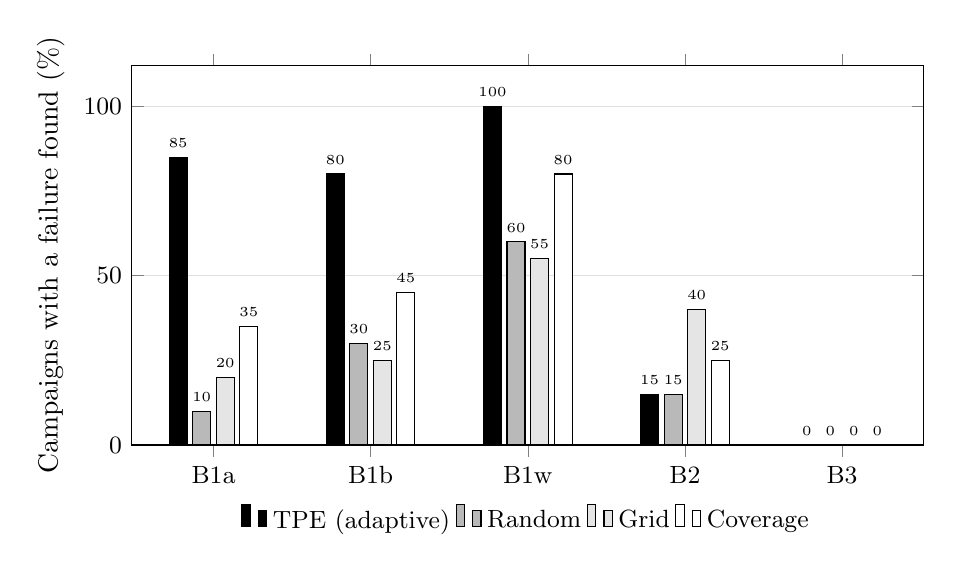
\begin{tikzpicture}
\begin{axis}[ybar, bar width=6.5pt, width=0.96\linewidth, height=6.4cm, ymin=0, ymax=112, ylabel={Campaigns with a failure found (\%)},
  symbolic x coords={B1a,B1b,B1w,B2,B3}, xtick=data, enlarge x limits=0.13, ymajorgrids, grid style={gray!25},
  legend style={at={(0.5,-0.14)},anchor=north,legend columns=4,draw=none,font=\small},
  nodes near coords, every node near coord/.append style={font=\tiny}, tick label style={font=\small}]
\addplot[fill=black,draw=black] coordinates {(B1a,85)(B1b,80)(B1w,100)(B2,15)(B3,0)};
\addplot[fill=gray!55,draw=black] coordinates {(B1a,10)(B1b,30)(B1w,60)(B2,15)(B3,0)};
\addplot[fill=gray!20,draw=black] coordinates {(B1a,20)(B1b,25)(B1w,55)(B2,40)(B3,0)};
\addplot[fill=white,draw=black] coordinates {(B1a,35)(B1b,45)(B1w,80)(B2,25)(B3,0)};
\legend{TPE (adaptive), Random, Grid, Coverage}
\end{axis}
\end{tikzpicture}\\[2pt]
{\setstretch{1}\small\itshape Figure 6.1: Campaigns that found a failure within 50 experiments, by planner and simulated profile (20 campaigns per cell).}
\end{figure}

\par\nopagebreak\noindent{\setstretch{1}\small\bfseries Table 6.2: Success within 30 and within 50 experiments (percent of 20 campaigns)}\par\nopagebreak\vspace{2pt}
\renewcommand{\arraystretch}{1.4}
\begin{longtable}{|>{\raggedright\arraybackslash\setlength{\parskip}{0pt}\setstretch{1}\small\bfseries}p{0.14\linewidth}|>{\centering\arraybackslash\setlength{\parskip}{0pt}\setstretch{1}\small}p{0.17\linewidth}|>{\centering\arraybackslash\setlength{\parskip}{0pt}\setstretch{1}\small}p{0.17\linewidth}|>{\centering\arraybackslash\setlength{\parskip}{0pt}\setstretch{1}\small}p{0.17\linewidth}|>{\centering\arraybackslash\setlength{\parskip}{0pt}\setstretch{1}\small}p{0.17\linewidth}|}
\hline
\rowcolor{ghead}\bfseries Profile & \bfseries TPE & \bfseries Random & \bfseries Grid & \bfseries Coverage \\ \hline
B1a & 65 / 85 & 10 / 10 & 20 / 20 & 20 / 35 \\ \hline
B1b & 55 / 80 & 25 / 30 & 15 / 25 & 30 / 45 \\ \hline
B1w & 90 / 100 & 40 / 60 & 25 / 55 & 60 / 80 \\ \hline
B2 & 15 / 15 & 5 / 15 & 15 / 40 & 5 / 25 \\ \hline
B3 (no fault) & 0 / 0 & 0 / 0 & 0 / 0 & 0 / 0 \\ \hline
\end{longtable}

TPE reached a failure within 50 experiments in 100\% of campaigns on B1w against 60\% for random, 85\% against 10\% on B1a and 80\% against 30\% on B1b. On B2, where the reset has no measurable precursor, TPE did not beat random (15\% each) and a grid did best (40\%), so the adaptive advantage depends on a precursor being visible. On B3, which has no fault, no planner reported a failure in any of 20 campaigns, so no false failures were raised. A fixed-corner baseline found nothing on any profile. With 20 campaigns per cell the 95\% Wilson intervals are wide (for example TPE on B1w within 50 experiments: 83.9 to 100\%, random: 38.7 to 78.1\%), and the numbers come from a simulator, so they indicate a trend that the repeated-seed evaluation of Section 8 must confirm.

\bluesub{6.3 Operator Console in Operation}
The screenshots below were taken from the Console running a demonstration of the OLED rig on the simulated bench with dummy data. The Console lists campaigns and their state, shows each approved contract with its requirements, observations and safety limits, follows a running campaign live with its outcome timeline and event log, reports results, and compares planners on the same contract. About 50 further screenshots (arming checklist, live view, episodes, fixtures, manual challenge and a mobile layout) are kept in the project repository.

\begin{figure}[t]
\centering
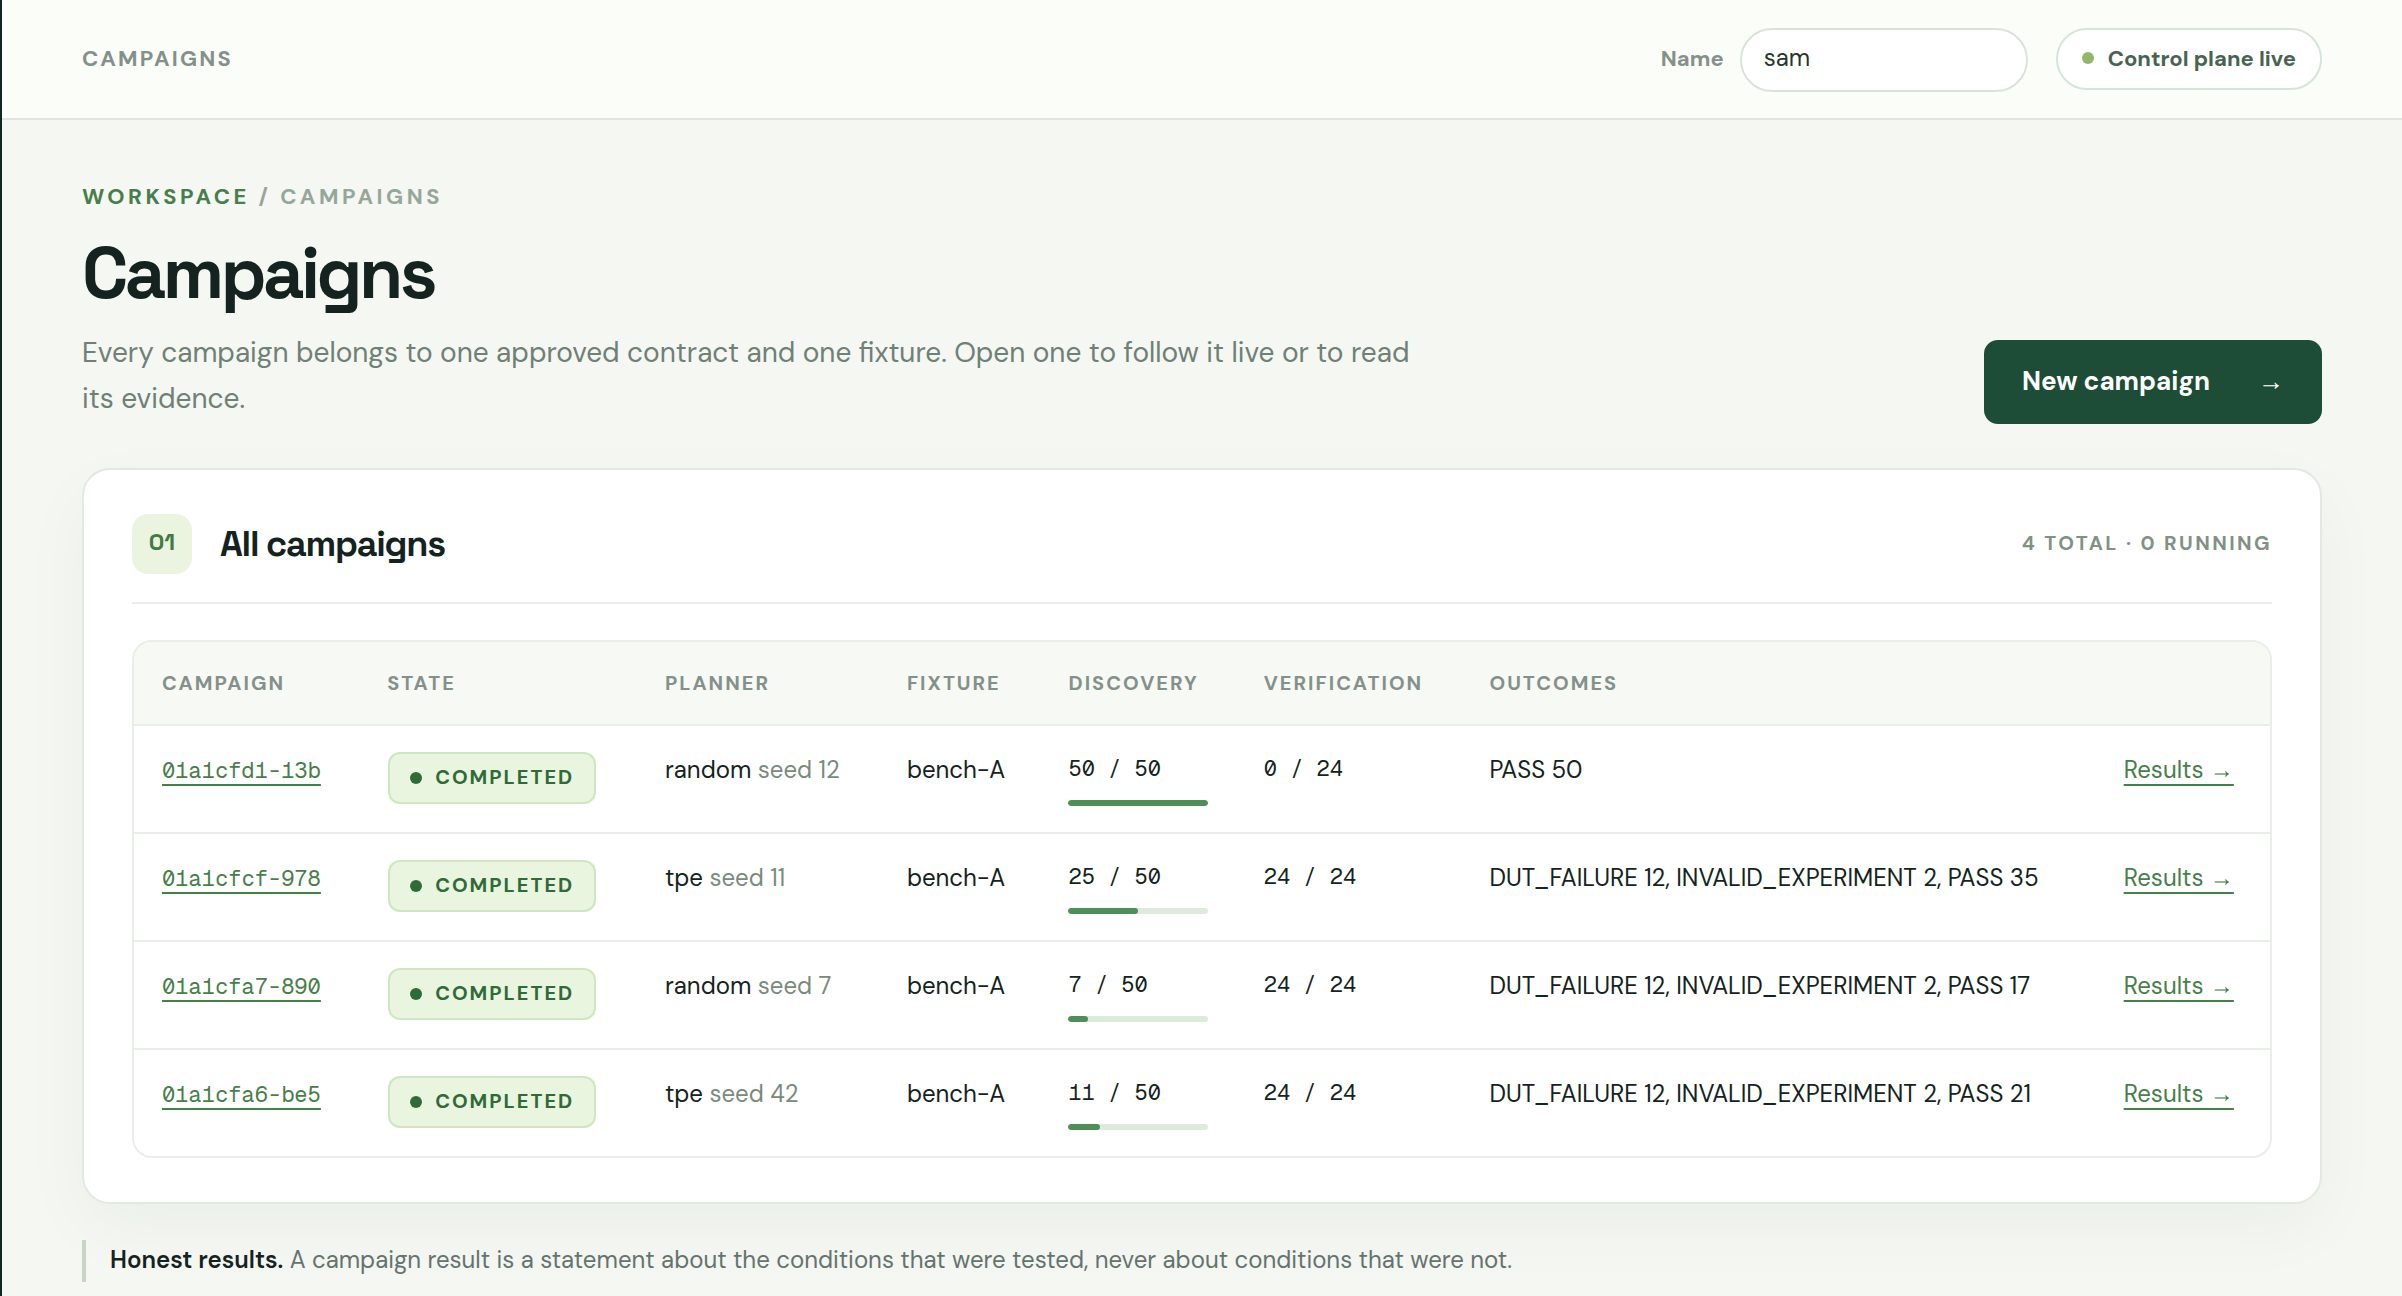
\includegraphics[width=0.93\linewidth]{figures/crop-console-list.png}\\[2pt]
{\setstretch{1}\small\itshape Figure 6.2: Console: campaign list with four finished campaigns, their state, planner, seed, budget use and outcome counts.}
\end{figure}

\begin{figure}[t]
\centering
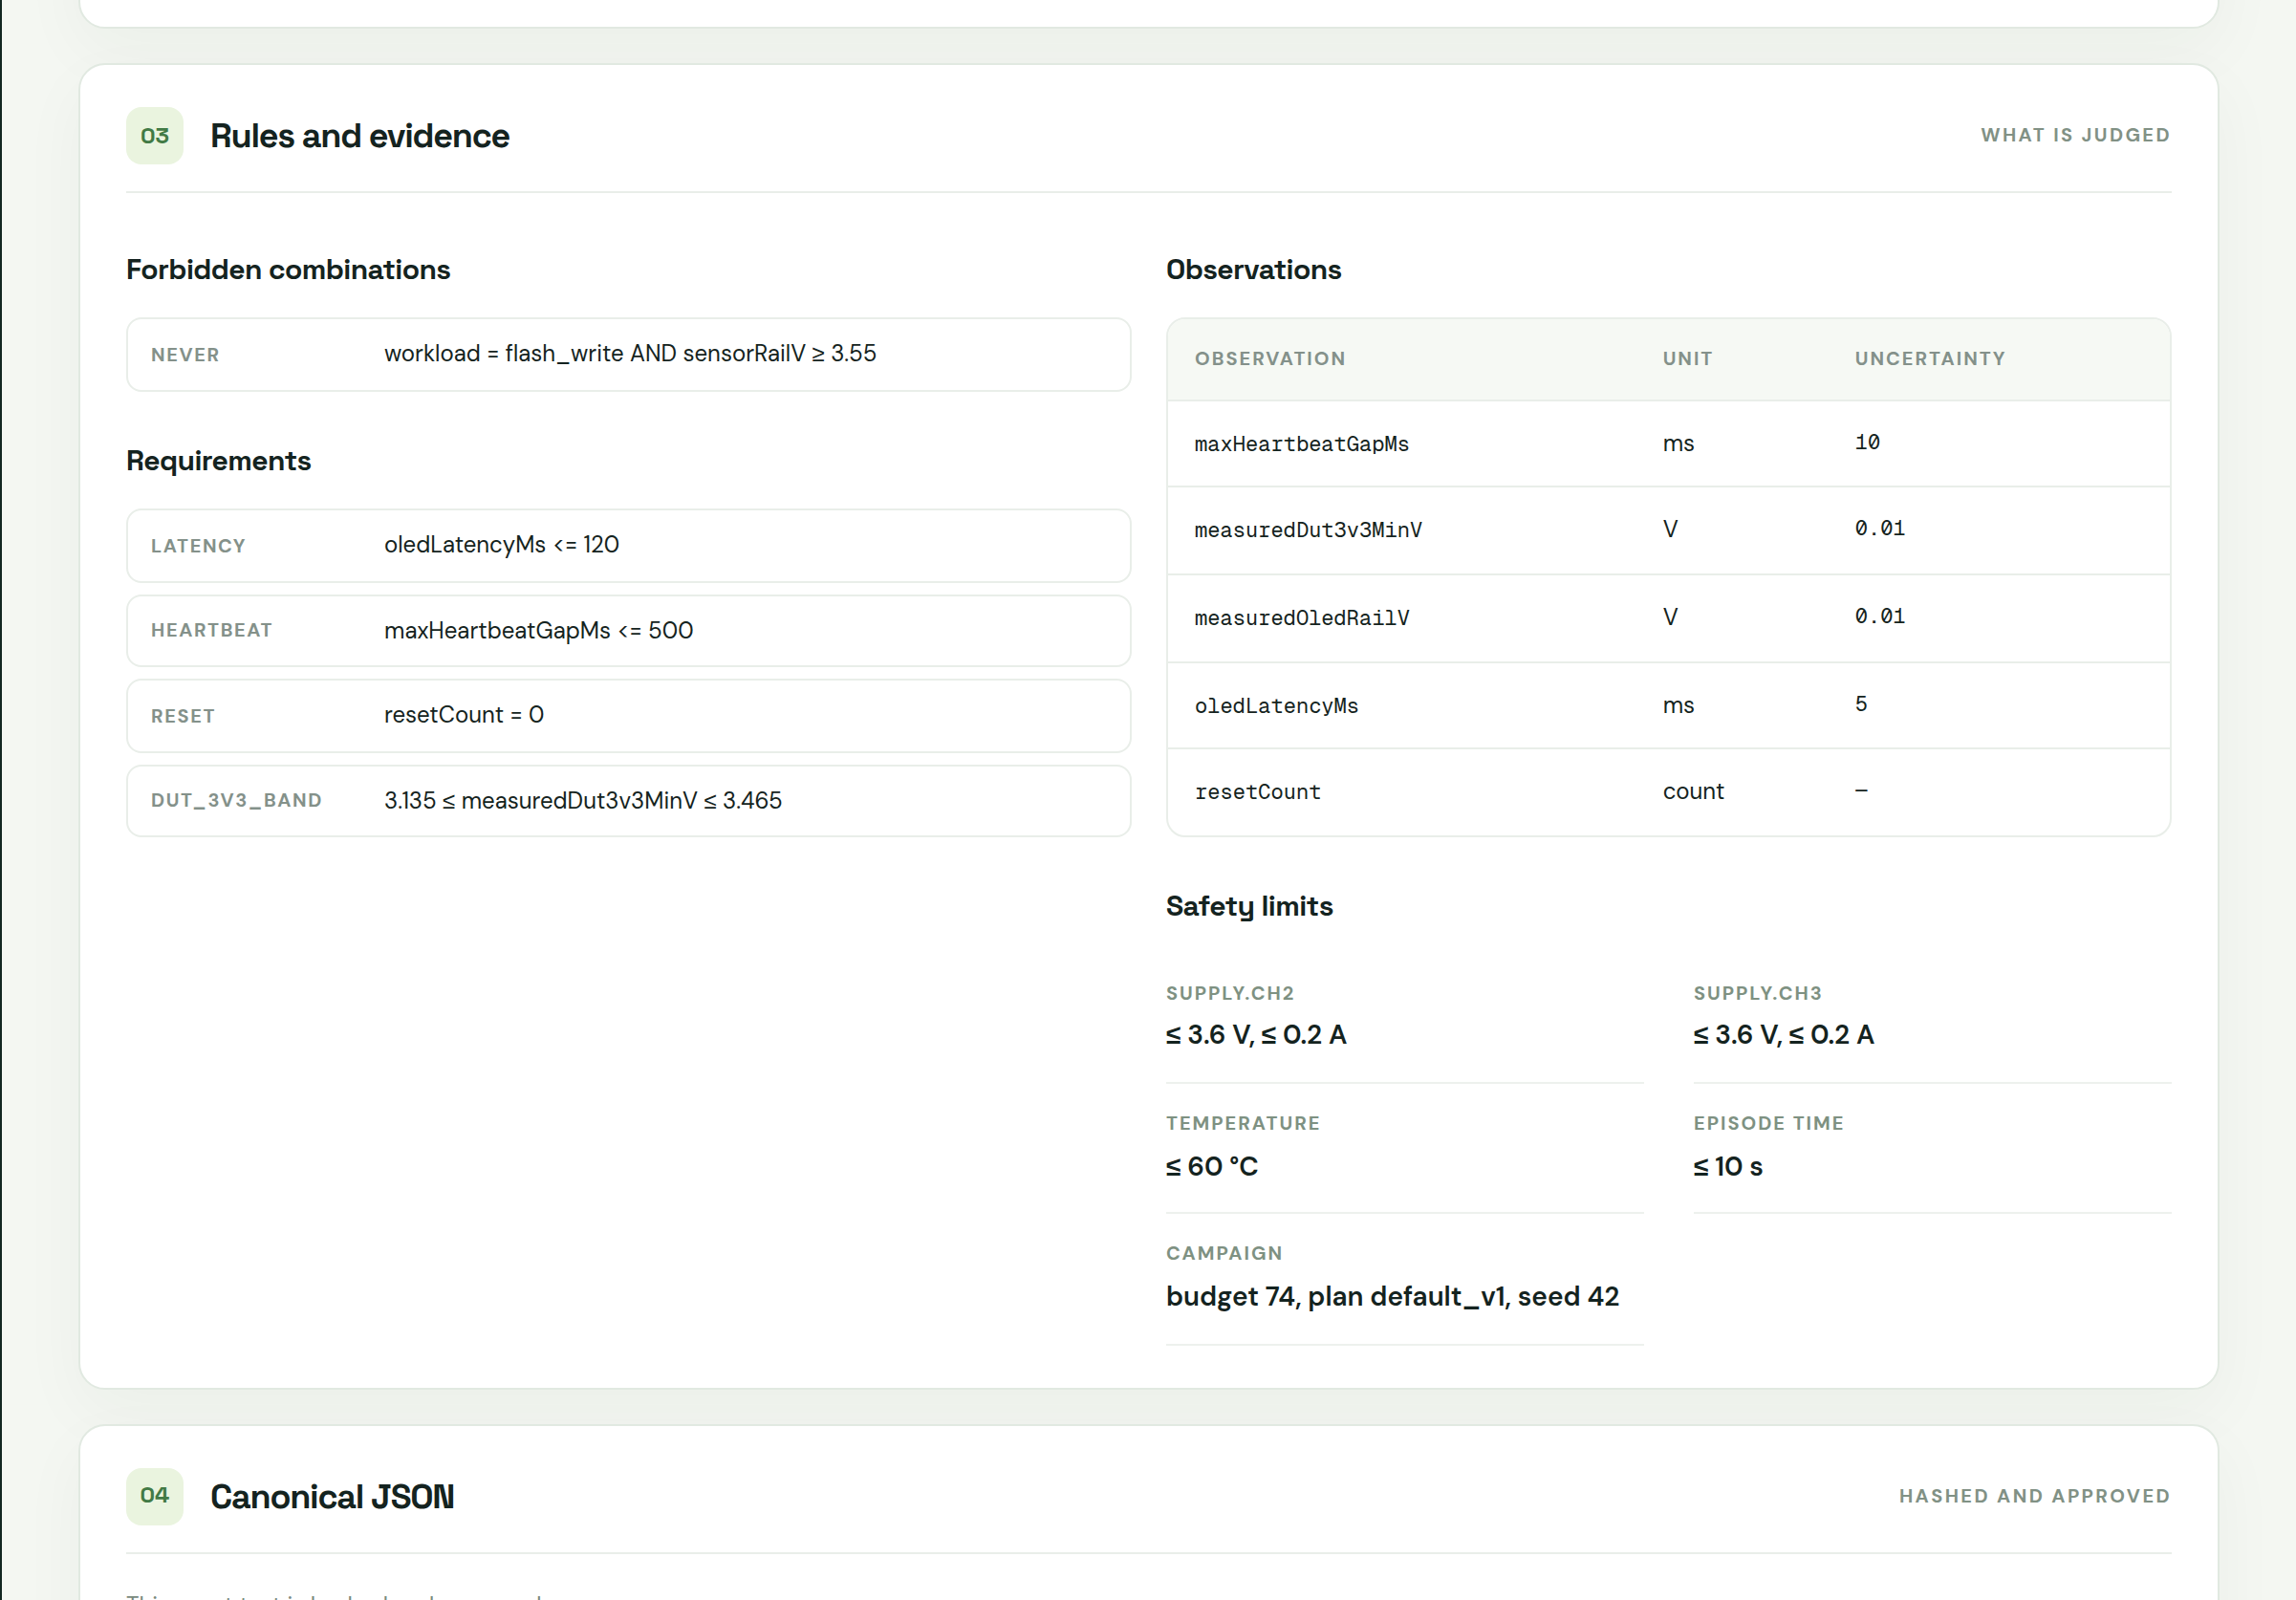
\includegraphics[width=0.93\linewidth]{figures/crop-console-2.png}\\[2pt]
{\setstretch{1}\small\itshape Figure 6.3: Console: an approved contract showing forbidden combinations, requirements, observations with their uncertainties and the hard safety limits.}
\end{figure}

\begin{figure}[t]
\centering
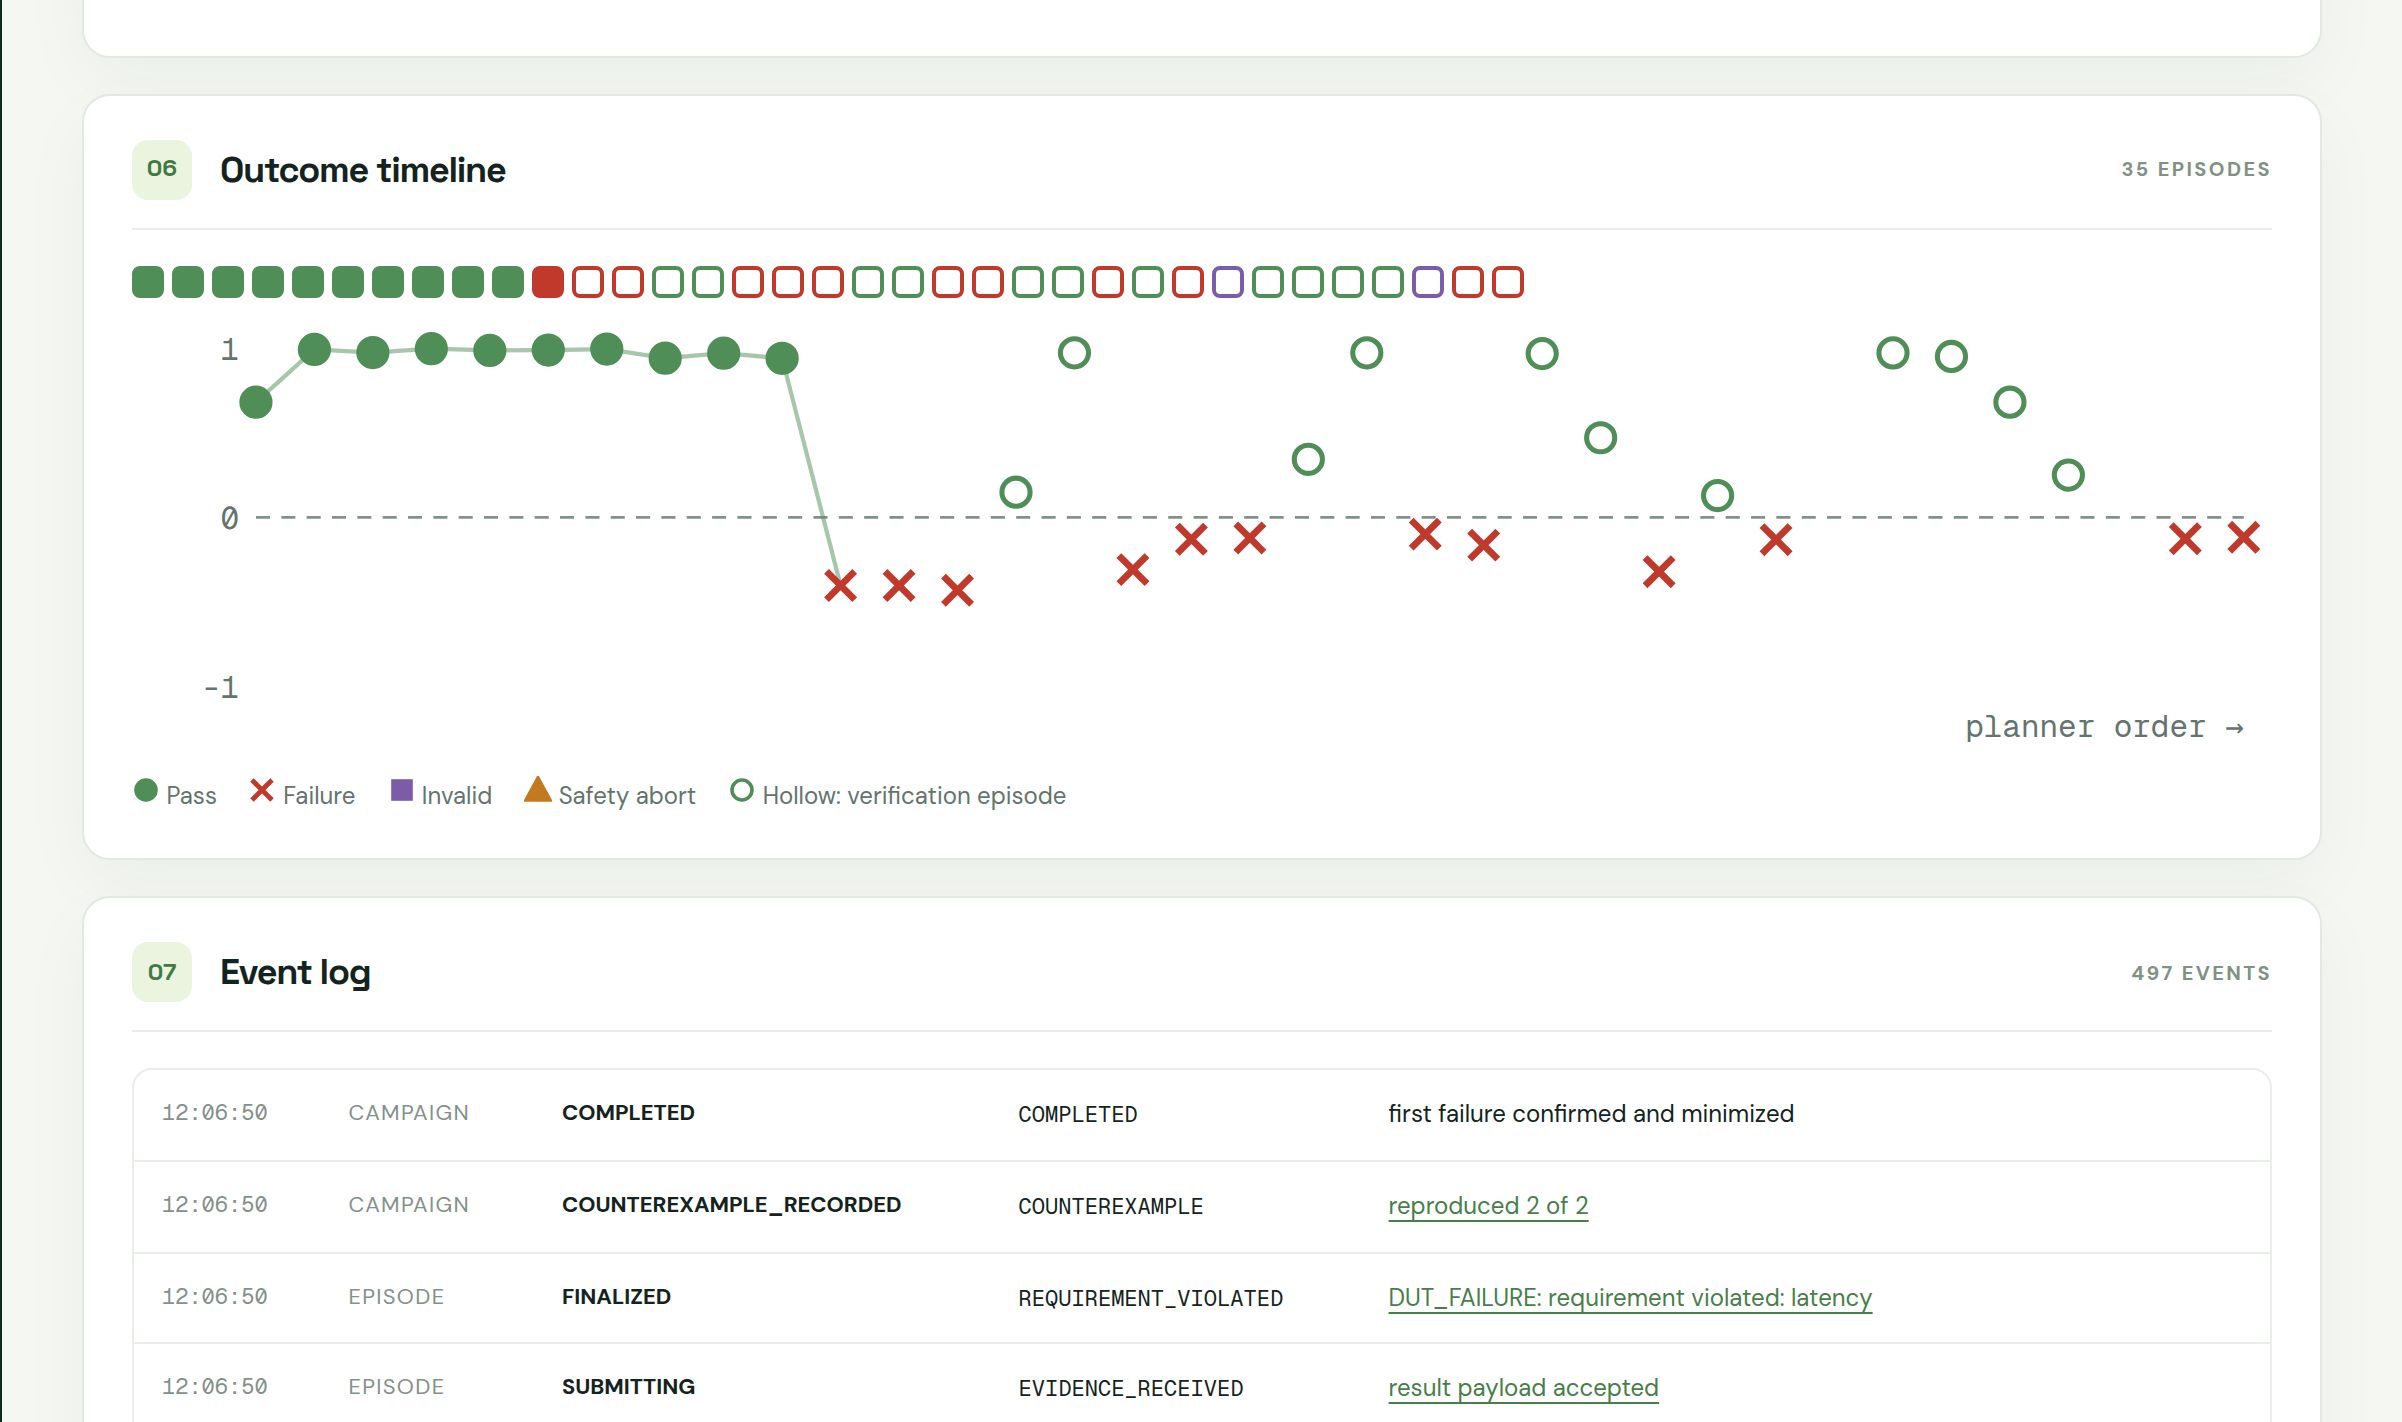
\includegraphics[width=0.93\linewidth]{figures/crop-console-3.png}\\[2pt]
{\setstretch{1}\small\itshape Figure 6.4: Console: the outcome timeline of a finished campaign (passes, failures, invalid episodes, and hollow marks for verification episodes) above the event log.}
\end{figure}

\begin{figure}[t]
\centering
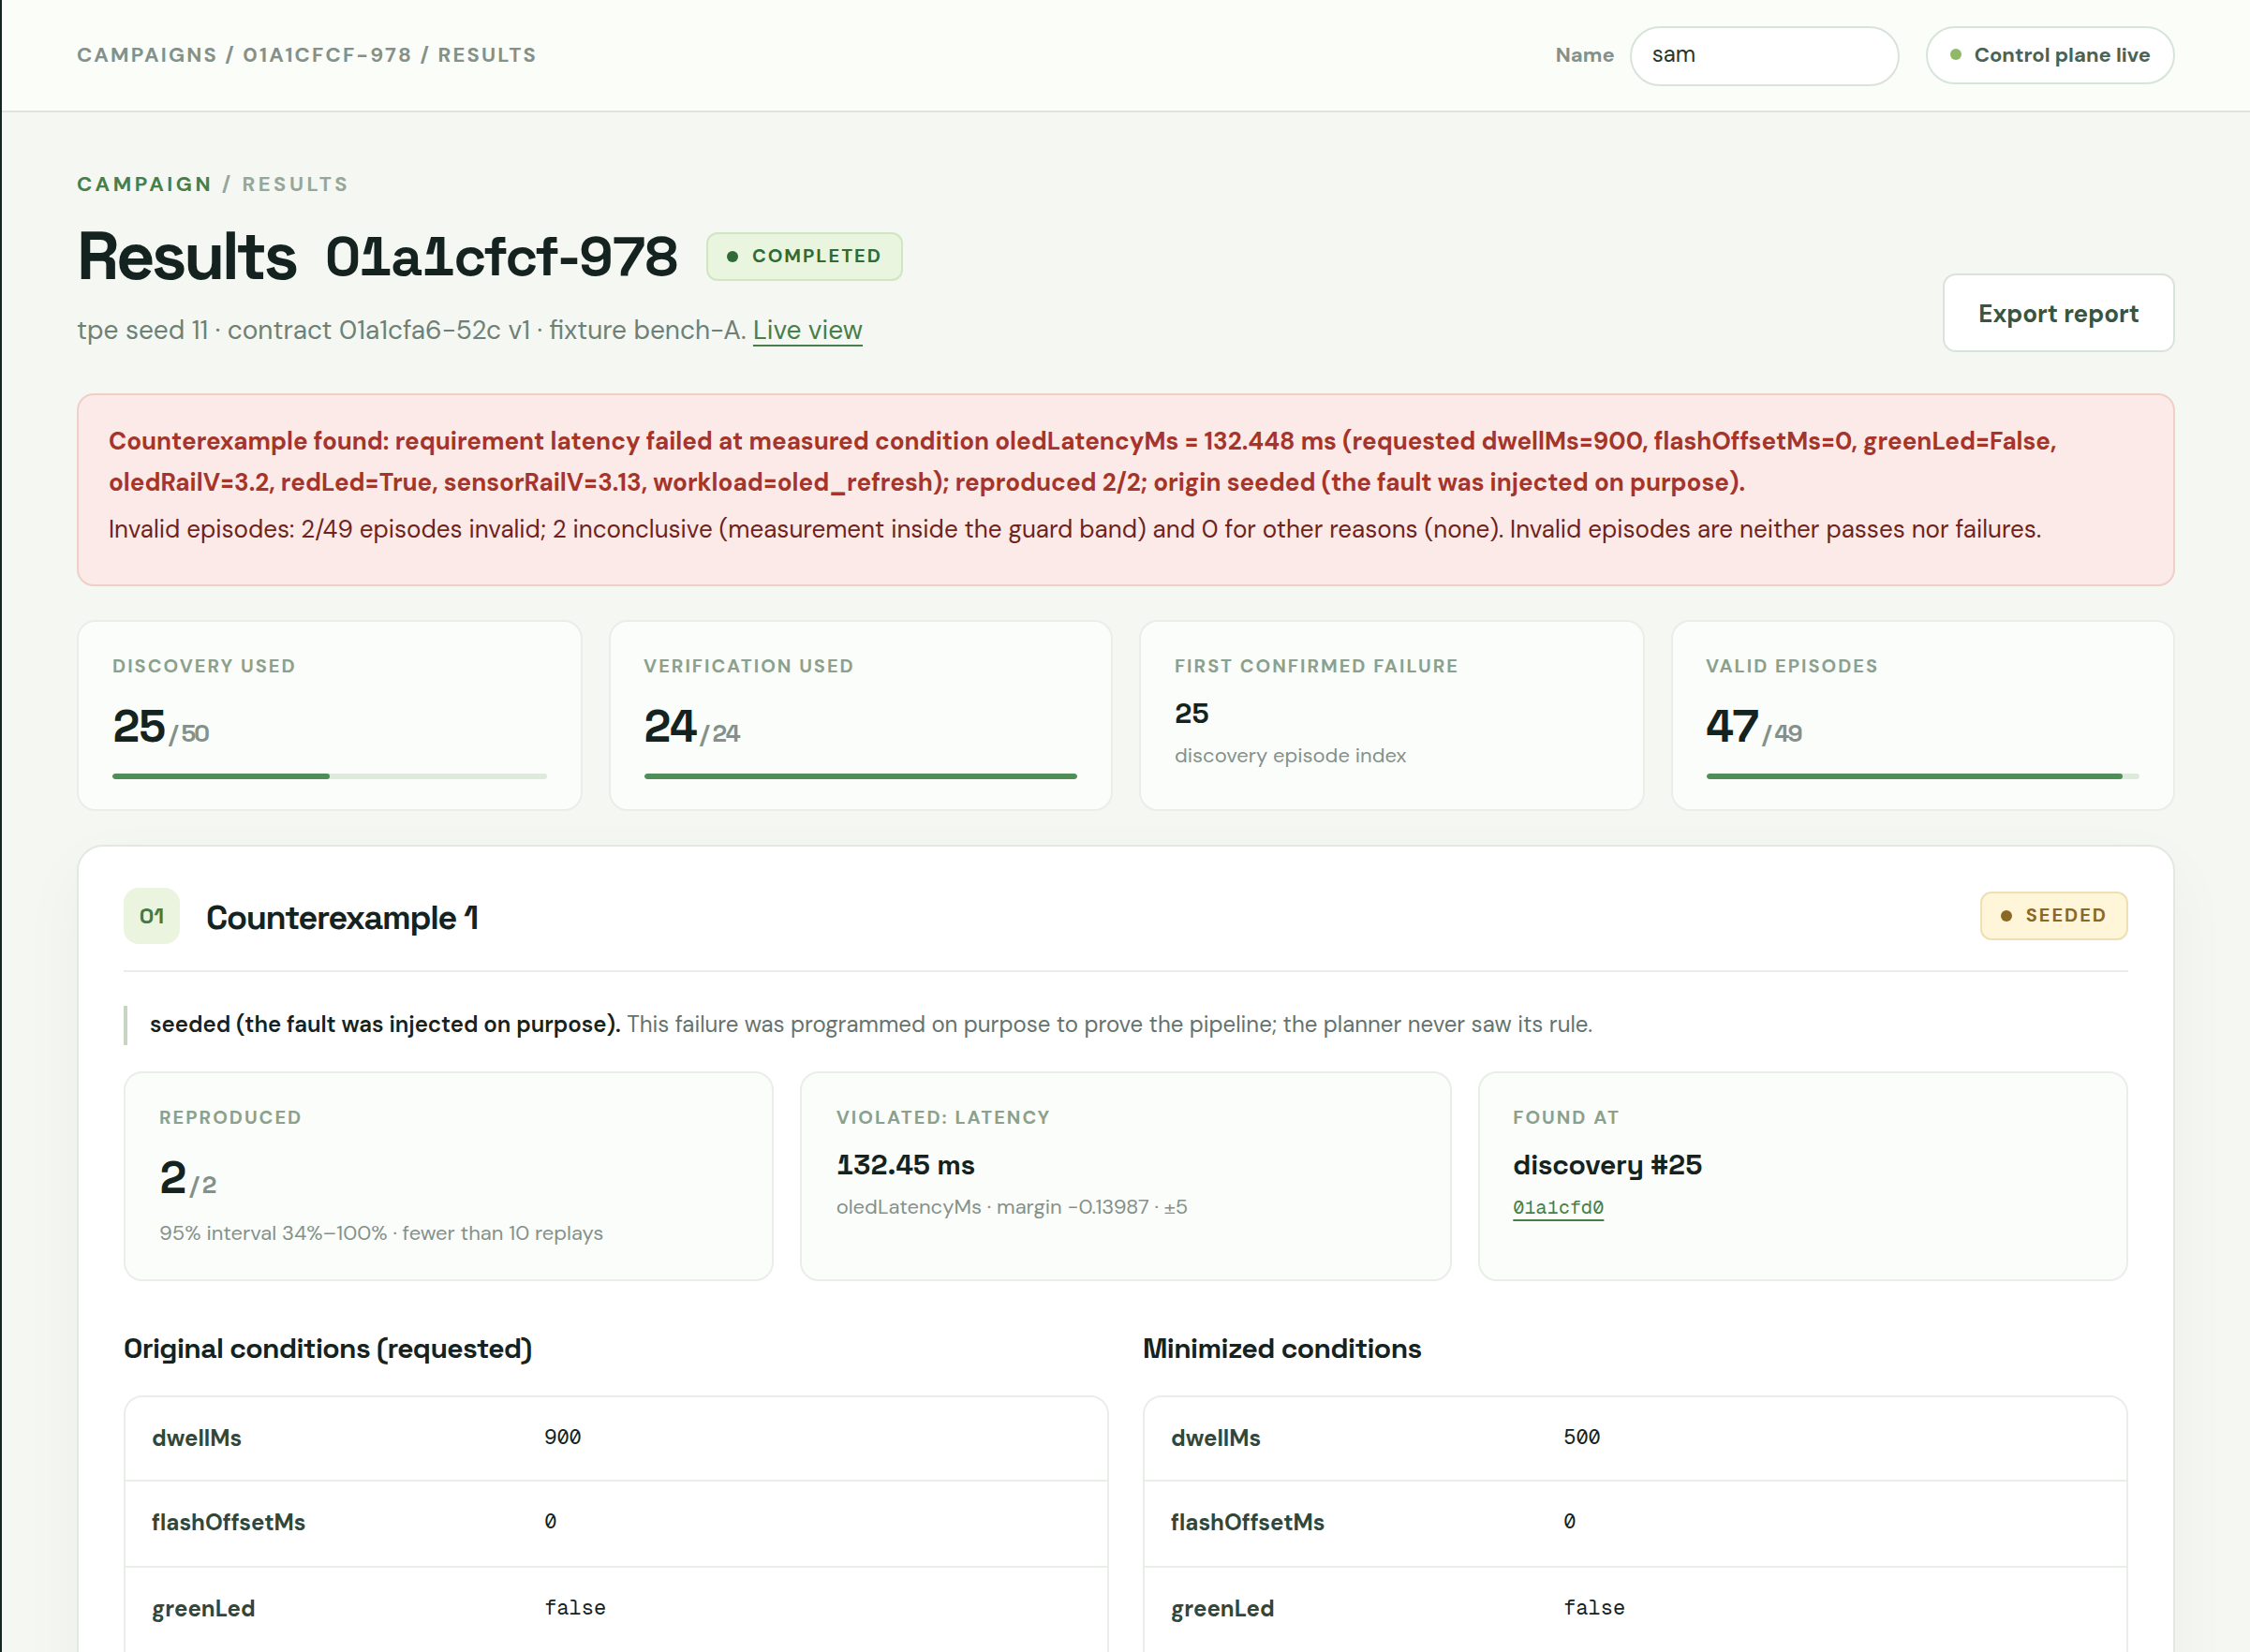
\includegraphics[width=0.93\linewidth]{figures/crop-console-results.png}\\[2pt]
{\setstretch{1}\small\itshape Figure 6.5: Console: results of a finished campaign. A counterexample is reported with its reproduction count, the violated requirement and the original and minimised conditions, and a failure injected on purpose is labelled as seeded.}
\end{figure}

\begin{figure}[t]
\centering
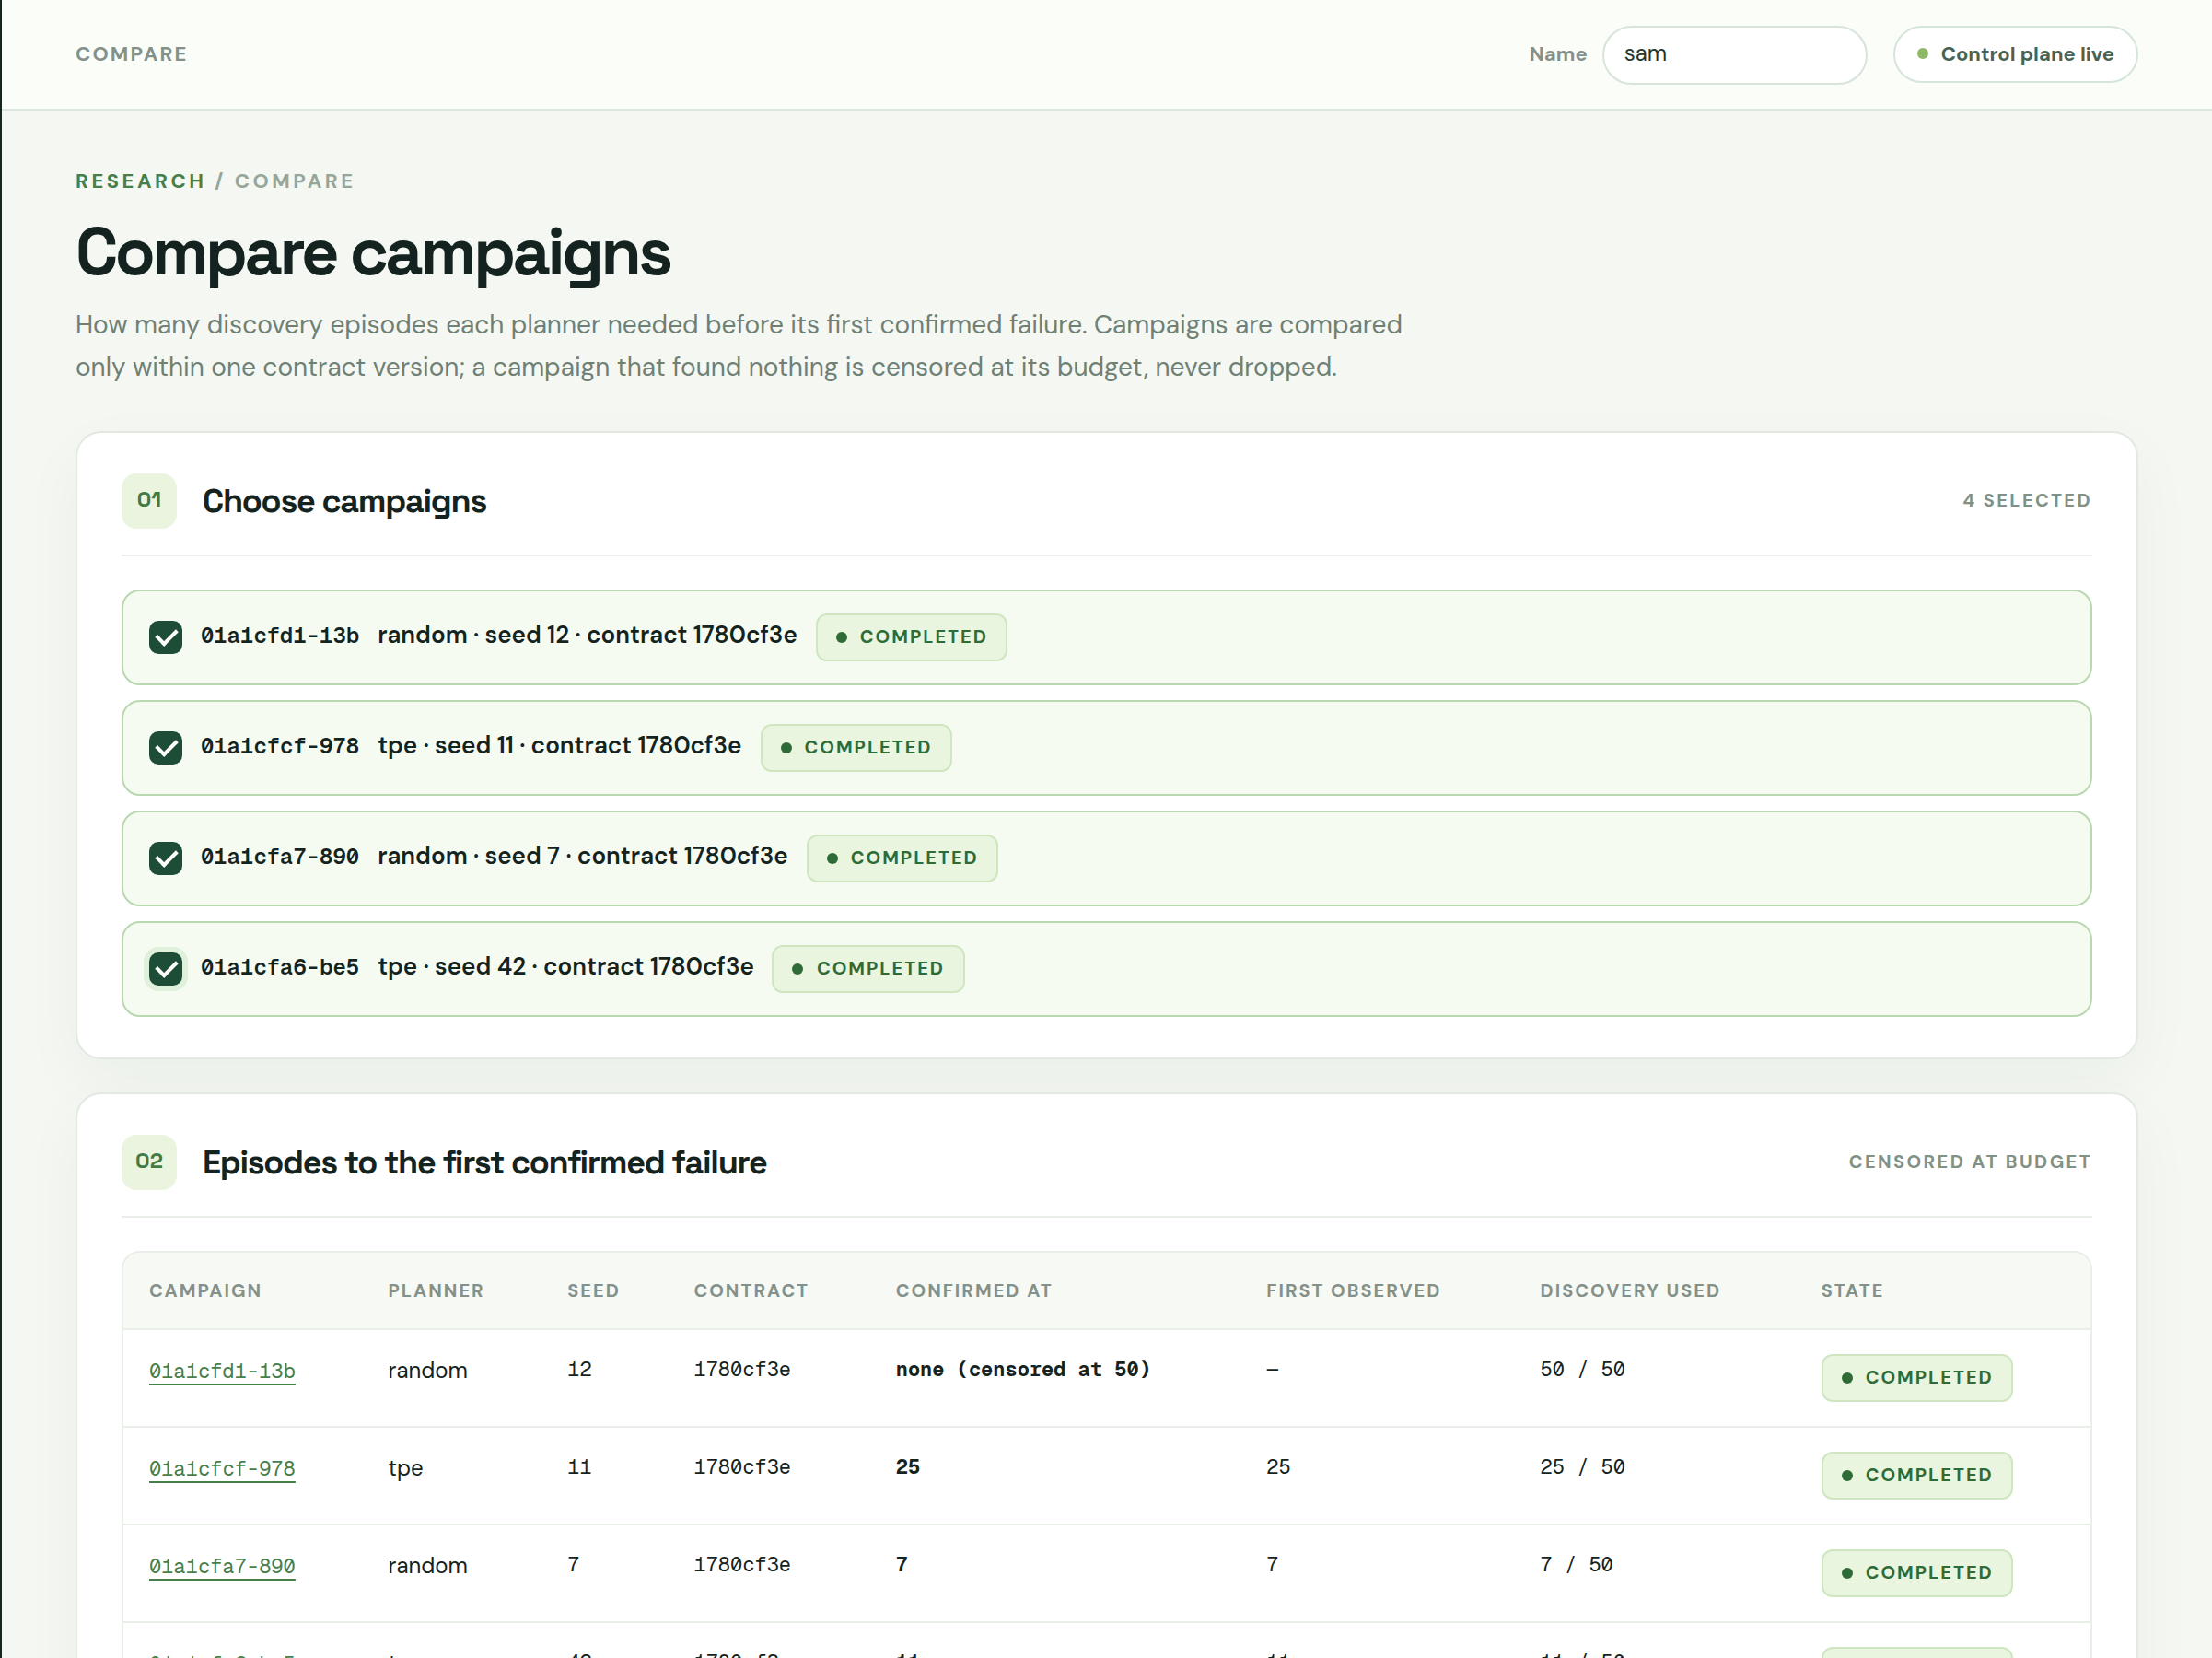
\includegraphics[width=0.93\linewidth]{figures/crop-console-4.png}\\[2pt]
{\setstretch{1}\small\itshape Figure 6.6: Console: comparison of planners on one contract. Episodes to the first confirmed failure are right-censored at the budget, so a campaign that found nothing in 50 episodes is shown as censored and not dropped.}
\end{figure}

\par\nopagebreak\noindent{\setstretch{1}\small\bfseries Table 6.3: Console demonstration campaigns (OLED rig, simulated bench)}\par\nopagebreak\vspace{2pt}
\renewcommand{\arraystretch}{1.4}
\begin{longtable}{|>{\raggedright\arraybackslash\setlength{\parskip}{0pt}\setstretch{1}\small\bfseries}p{0.18\linewidth}|>{\raggedright\arraybackslash\setlength{\parskip}{0pt}\setstretch{1}\small}p{0.24\linewidth}|>{\centering\arraybackslash\setlength{\parskip}{0pt}\setstretch{1}\small}p{0.13\linewidth}|>{\centering\arraybackslash\setlength{\parskip}{0pt}\setstretch{1}\small}p{0.08\linewidth}|>{\centering\arraybackslash\setlength{\parskip}{0pt}\setstretch{1}\small}p{0.09\linewidth}|>{\centering\arraybackslash\setlength{\parskip}{0pt}\setstretch{1}\small}p{0.08\linewidth}|}
\hline
\rowcolor{ghead}\bfseries Campaign & \bfseries First confirmed failure & \bfseries Discovery used & \bfseries Fail & \bfseries Invalid & \bfseries Pass \\ \hline
TPE, seed 42 & episode 11 & 11 / 50 & 12 & 2 & 21 \\ \hline
TPE, seed 11 & episode 25 & 25 / 50 & 12 & 2 & 35 \\ \hline
Random, seed 7 & episode 7 & 7 / 50 & 12 & 2 & 17 \\ \hline
Random, seed 12 & none (censored at 50) & 50 / 50 & 0 & 0 & 50 \\ \hline
\end{longtable}

Failure counts include the verification episodes used to confirm and minimise a failure. One campaign per planner proves nothing: a log-rank test of random against TPE on these four runs gives $p = 0.69$, so no difference is claimed. The repeated seeds of the final evaluation are pre-registered for that purpose.

\bluesub{6.4 Timing Test on the ESP32 Bench Model}
Figure 6.7 shows the isometric bench model running three experiments of the timing feature. The deadline rule of Section 5.3 is applied to each scheduled task release, and the laptop screen in the model draws how late each task finished against its deadline. The counts in Table 6.4 come from the timing model that drives the figure, not from a physical board.

\begin{figure}[t]
\centering
\begin{minipage}{0.325\linewidth}\centering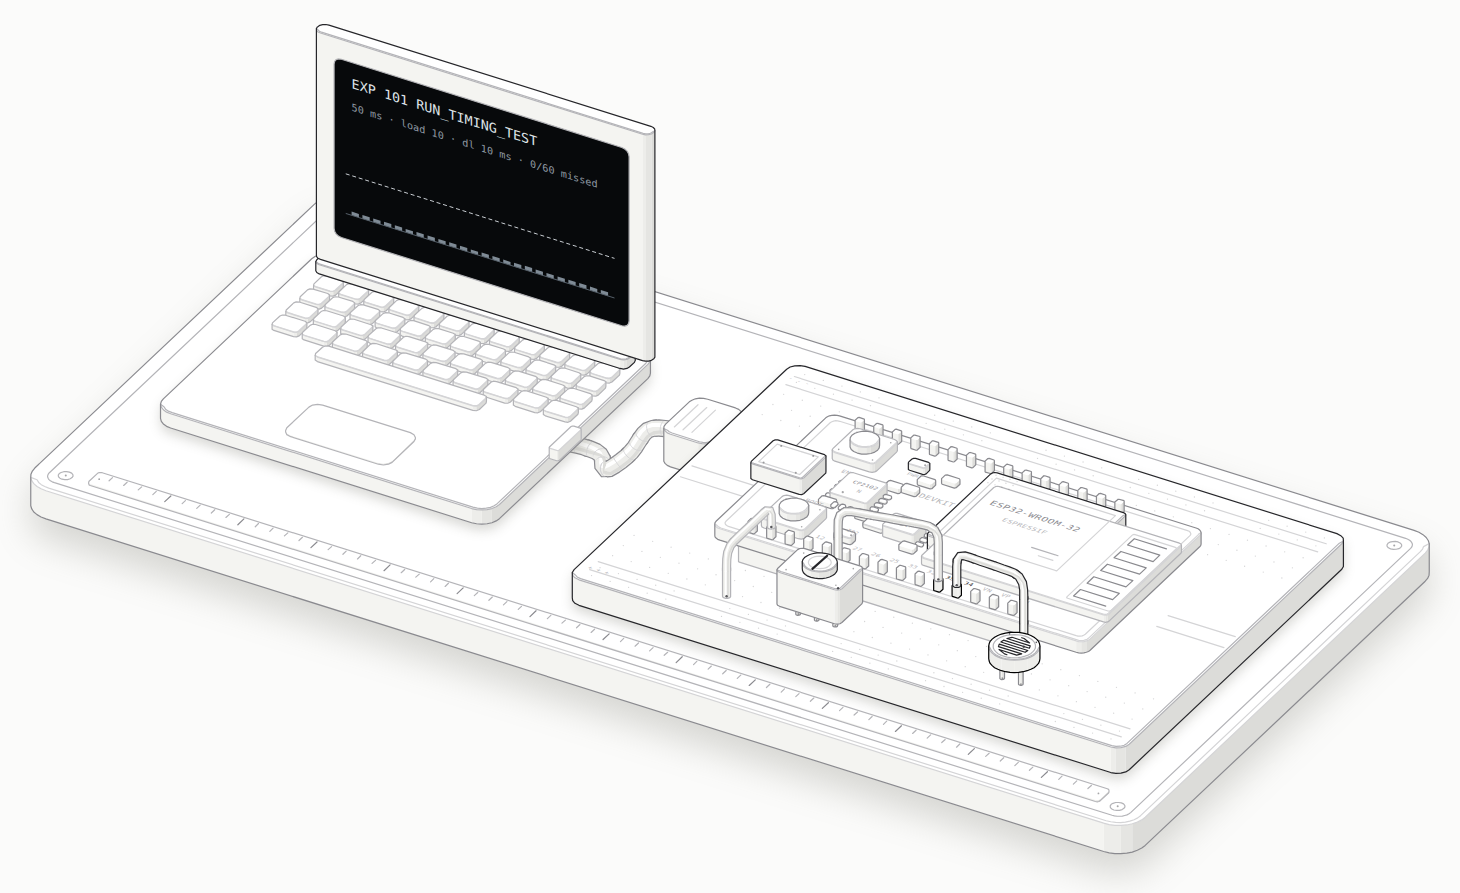
\includegraphics[width=\linewidth]{figures/crop-bench-pass.png}\\{\setstretch{1}\scriptsize\itshape (a) Nominal: PASS}\end{minipage}\hfill
\begin{minipage}{0.325\linewidth}\centering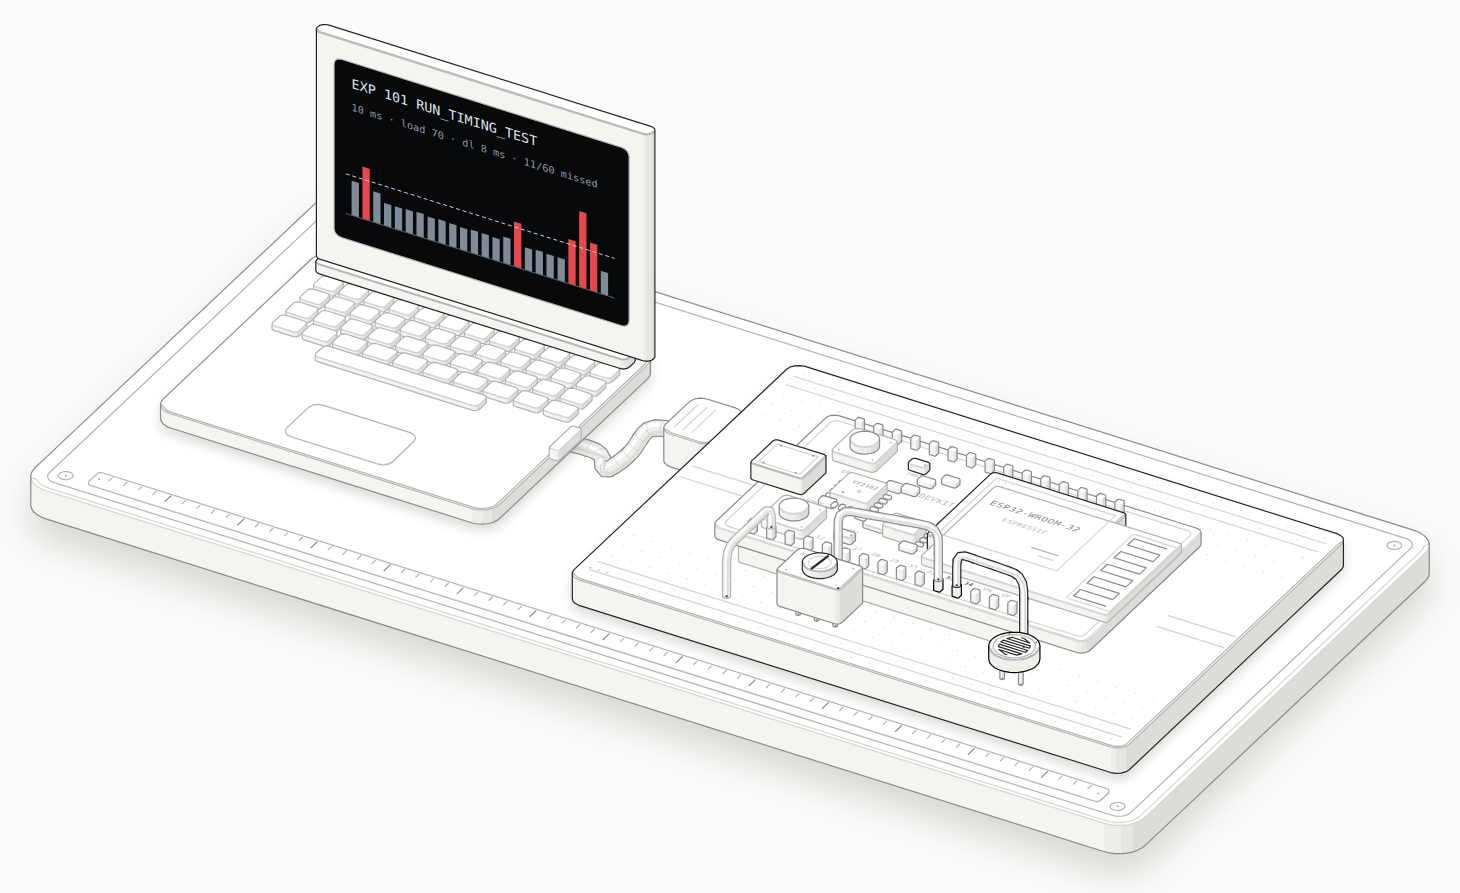
\includegraphics[width=\linewidth]{figures/crop-bench-defA.png}\\{\setstretch{1}\scriptsize\itshape (b) Seeded defect A: TIMING\_FAILURE}\end{minipage}\hfill
\begin{minipage}{0.325\linewidth}\centering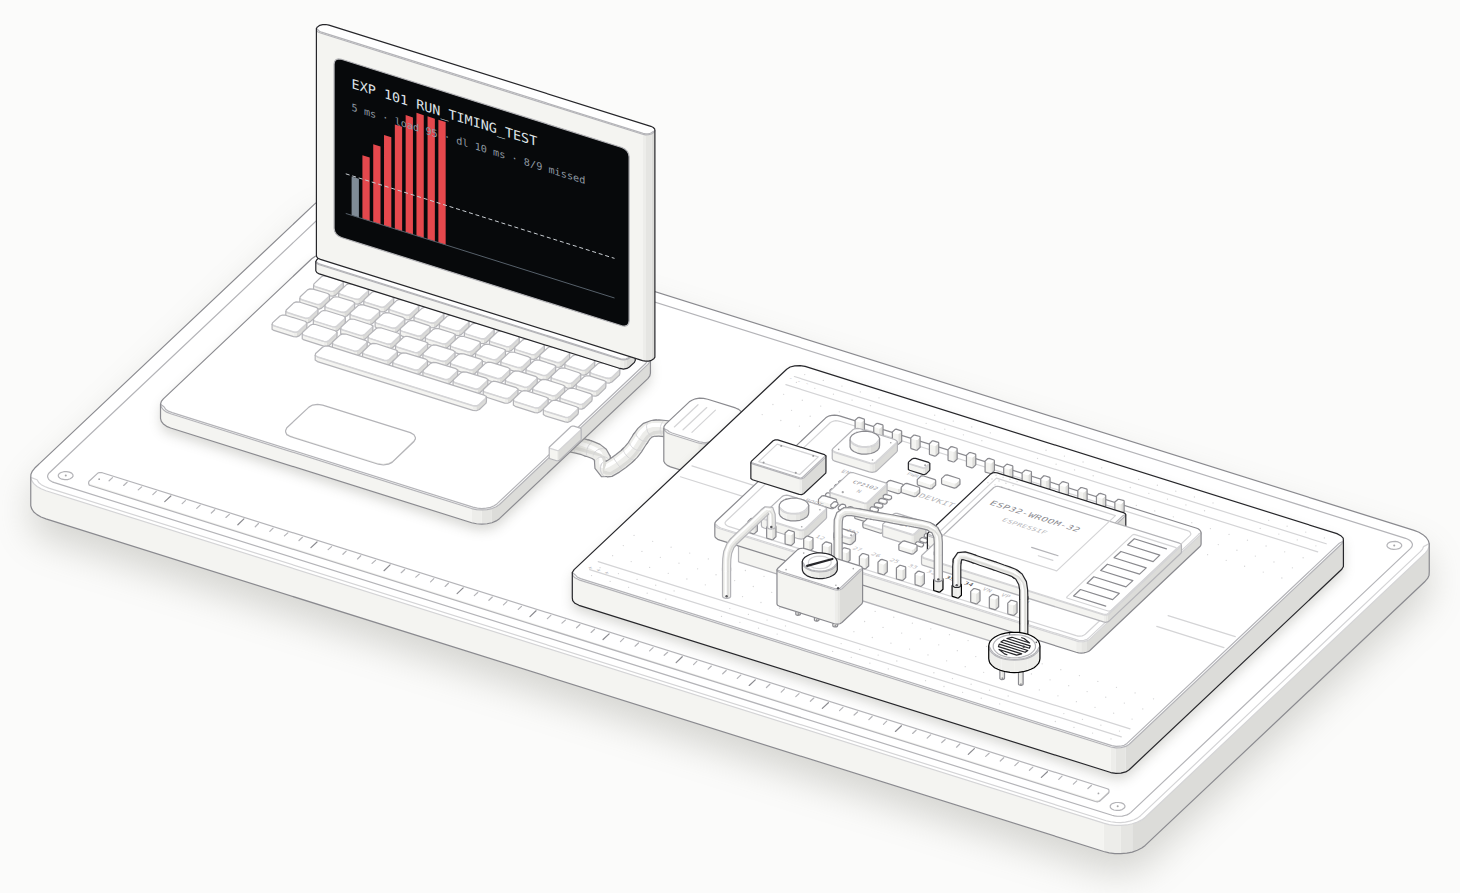
\includegraphics[width=\linewidth]{figures/crop-bench-defC.png}\\{\setstretch{1}\scriptsize\itshape (c) Seeded defect C: WATCHDOG\_RESET}\end{minipage}\\[4pt]
{\setstretch{1}\small\itshape Figure 6.7: The bench model in three experiments. Missed deadlines are the dark bars above the dashed deadline line on the laptop screen.}
\end{figure}

\par\nopagebreak\noindent{\setstretch{1}\small\bfseries Table 6.4: Timing experiments on the bench model (60 scheduled releases)}\par\nopagebreak\vspace{2pt}
\renewcommand{\arraystretch}{1.4}
\begin{longtable}{|>{\raggedright\arraybackslash\setlength{\parskip}{0pt}\setstretch{1}\small\bfseries}p{0.19\linewidth}|>{\centering\arraybackslash\setlength{\parskip}{0pt}\setstretch{1}\small}p{0.10\linewidth}|>{\centering\arraybackslash\setlength{\parskip}{0pt}\setstretch{1}\small}p{0.08\linewidth}|>{\centering\arraybackslash\setlength{\parskip}{0pt}\setstretch{1}\small}p{0.11\linewidth}|>{\centering\arraybackslash\setlength{\parskip}{0pt}\setstretch{1}\small}p{0.12\linewidth}|>{\raggedright\arraybackslash\setlength{\parskip}{0pt}\setstretch{1}\small\ttfamily}p{0.21\linewidth}|}
\hline
\rowcolor{ghead}\bfseries Experiment & \bfseries Interval & \bfseries Load & \bfseries Deadline & \bfseries Missed & \bfseries\rmfamily Outcome \\ \hline
Nominal & 50 ms & 10 & 10 ms & 0 of 60 & PASS \\ \hline
Seeded defect A & 10 ms & 70 & 8 ms & 11 of 60 & TIMING\_FAILURE \\ \hline
Seeded defect C & 5 ms & 95 & 10 ms & 8 of 9 & WATCHDOG\_RESET \\ \hline
\end{longtable}

In the defect C run the model stops after nine releases because the simulated watchdog resets the board, which is why the experiment is labelled \texttt{WATCHDOG\_RESET} and not a deadline failure.

\bluesub{6.5 Discussion}
The partial results support three points. First, the loop is complete in simulation: contract, planner, two safety checks, execution, oracle, confirmation, minimisation and an evidence report all ran without an unsafe execution. Second, on profiles where a failure leaves a measurable precursor, TPE reached a failure in fewer experiments than random, grid and coverage selection. Third, on a profile with no precursor an adaptive method has no advantage, and on a fault-free profile none of the planners raised a false failure. The limits are equally clear: the results are simulated, the sample sizes are small, the ESP32 timing pipeline is still being integrated, and no physical measurement has been made yet.

\redsec{7. Expected Outcomes \& Deliverables}
\dredrule
Upon successful completion of this project, the following outcomes are expected:

\purpsub{7.1 Technical Outcomes}
\begin{itemize}
\item\relax A working testbench in which every candidate passes two independent safety checks, with zero rejected configurations executed in all campaigns.
\item\relax A JSON-Lines protocol and an ESP32 bring-up that return microsecond raw samples, with the PC recomputation agreeing with the firmware summary within the stated tolerances (0.05 ms for mean interval and jitter, 0.002 for miss rate) on a clean run, and a corrupted summary always detected.
\item\relax An adaptive planner, three ablations and four baselines on one loop, with identical output for identical seeds in simulation.
\item\relax A console with seven views (device status, experiment configuration, live monitor, results and raw telemetry, adaptive testing, research comparison and audit log) and CSV and JSON export of raw samples.
\end{itemize}

\purpsub{7.2 Research Outcomes}
\begin{itemize}
\item\relax Evidence, with confidence intervals over repeated seeds, on whether adaptive selection reaches the first timing failure and finds more distinct failure signatures than random and grid selection at equal budgets of 15, 30 and 50 experiments. The hypothesis that the median experiments-to-first-failure is at least 30\% lower than random is to be tested and may be rejected.
\item\relax An ablation showing which term of the acquisition matters, and a measured discrepancy rate for firmware self-reports.
\item\relax A reproducible open design and a paper draft, kept honest about simulation versus hardware and about what the absence of failures does not prove.
\end{itemize}

\purpsub{7.3 Deliverables Checklist}
\par\nopagebreak\noindent{\setstretch{1}\small\bfseries Table 7.1: Deliverables and target timeline}\par\nopagebreak\vspace{2pt}
\renewcommand{\arraystretch}{1.5}
\begin{longtable}{|>{\raggedright\arraybackslash\setlength{\parskip}{0pt}\setstretch{1}\small}p{0.55\linewidth}|>{\raggedright\arraybackslash\setlength{\parskip}{0pt}\setstretch{1}\small}p{0.345\linewidth}|}
\hline
\rowcolor{ghead}\bfseries Deliverable & \bfseries Target Timeline \\ \hline
Synopsis / Proposal Document & Week 2 \\ \hline
Literature Review Report & Week 2 \\ \hline
Simulator, Planner Interface and Baseline Planners & Week 4 \\ \hline
Safe Bench with ESP32 Firmware and Bring-up Evidence & Week 8 \\ \hline
Integrated Adaptive Campaigns, Console and Code Repository & Week 10 \\ \hline
Evaluation Report \& Results & Week 12 \\ \hline
Final Project Report, Paper Draft \& Presentation & Week 13 \\ \hline
\end{longtable}

\purpsec{8. Evaluation Metrics \& Validation Plan}
\dredrule
\Needspace{14\baselineskip}
\textbf{Research questions.}
\par\nopagebreak\noindent{\setstretch{1}\small\bfseries Table 8.1: Research questions and hypotheses (to be pre-registered before the final runs)}\par\nopagebreak\vspace{2pt}
\renewcommand{\arraystretch}{1.4}
\begin{longtable}{|>{\raggedright\arraybackslash\setlength{\parskip}{0pt}\setstretch{1}\small\bfseries}p{0.10\linewidth}|>{\raggedright\arraybackslash\setlength{\parskip}{0pt}\setstretch{1}\small}p{0.43\linewidth}|>{\raggedright\arraybackslash\setlength{\parskip}{0pt}\setstretch{1}\small}p{0.37\linewidth}|}
\hline
\rowcolor{ghead}\bfseries ID & \bfseries Question & \bfseries Hypothesis \\ \hline
RQ-T1 & Does the full adaptive strategy reach the first timing failure in fewer experiments than random and grid at equal budget? & Median experiments-to-first-failure is at least 30\% lower than random (may be rejected) \\ \hline
RQ-T2 & Does it find more distinct failure signatures per budget? & Higher unique-signature count at budgets 15, 30 and 50 \\ \hline
RQ-T3 & Which acquisition term matters? & Removing failure probability hurts most; removing novelty lowers diversity \\ \hline
RQ-T4 & Are firmware self-reports trustworthy? & Discrepancy rate near zero on healthy hardware; injected corruption always detected \\ \hline
RQ-T5 & Do simulator conclusions transfer to hardware? & Exploratory; reported as such \\ \hline
\end{longtable}

\textbf{Metrics:}
\begin{itemize}
\item\relax \emph{Primary:} discovery rate at budget; experiments to the first failure, right-censored at the budget; number of unique failure signatures; discovery curve (unique failures against experiments); time to first failure measured as cumulative experiment time and not as wall-clock time.
\item\relax \emph{Secondary:} mean deadline-miss rate and jitter of executed experiments, count of rejected configurations, discrepancy count, planner compute time.
\item\relax \emph{Safety and integrity:} number of unsafe or rejected configurations executed (target exactly zero), discrepancy detection of injected corruption, and symmetric rejection by both the PC and the device.
\end{itemize}

\textbf{Validation strategy:}
\begin{itemize}
\item\relax Strategies: the full planner, three ablations, random, grid, TPE and space-filling selection, all on the same device, fault configuration, noise-seed policy and oracle, with the order of strategies randomised on hardware.
\item\relax Budgets of 15, 30 and 50 experiments, with at least 30 independent seeds per strategy and budget where time allows.
\item\relax Medians and interquartile ranges with 95\% bootstrap confidence intervals, Kaplan--Meier curves for censored time to failure, and paired comparison on matched seeds with effect sizes. The primary metric is stated before the runs, oracle thresholds, tolerances and signature bucket widths are frozen before the final evaluation, all seeds and raw logs are published, and there is no tuning after the results are seen.
\item\relax Simulation and hardware results are reported separately and labelled as such, and real-hardware evaluation starts only after the bring-up checklist (steps 1 to 13) passes.
\end{itemize}

\textbf{Threats to validity.} The seeded defects are artificial, and a small search space can favour a grid; both are disclosed and reported honestly. Calibrated work units may differ between boards, so each board is calibrated and the calibration is recorded. Timestamps come from the ESP32 clock and never from the host, so USB scheduling noise on the laptop does not enter any metric. Thermal and state drift on hardware is checked with a reference experiment between blocks and by logging boot identifiers and reset reasons.

\textbf{Ethical and safety considerations.}
\begin{itemize}
\item\relax No human subjects or personal data are involved.
\item\relax Version 1 adds no electrical hazard beyond USB-powered bench work, and the multi-rail rig keeps every supply within a reviewed extra-low-voltage envelope with a hardware cut-off.
\item\relax Results use honest language: a counterexample was found, or no failure was found within the budget. Neither is ever described as proof that the device is safe.
\end{itemize}

\purpsec{9. References}
\dredrule
\begingroup
\setstretch{1}\setlength{\parskip}{6pt}\sloppy\emergencystretch=3em\urlstyle{same}
\newcommand{\refitem}[1]{\par\noindent\hangindent=2.4em\hangafter=1 #1}
\vspace{4pt}
\refitem{[1]\hspace{0.5em}United Nations Department of Economic and Social Affairs, ``Goal 9: Industry, innovation and infrastructure,'' targets 9.1--9.c. [Online]. Available: \url{https://sdgs.un.org/goals/goal9}}

\refitem{[2]\hspace{0.5em}M. Zalewski, ``Technical whitepaper for afl-fuzz,'' AFL technical documentation. [Online]. Available: \url{https://github.com/google/AFL/blob/master/docs/technical_details.txt}}

\refitem{[3]\hspace{0.5em}J. Yun, F. Rustamov, J. Kim, and Y. Shin, ``Fuzzing of embedded systems: A survey,'' \textit{ACM Comput. Surv.}, vol. 55, no. 7, 2023. doi: 10.1145/3538644}

\refitem{[4]\hspace{0.5em}M. Eisele, M. Maugeri, R. Shriwas, C. Huth, and G. Bella, ``Embedded fuzzing: A review of challenges, tools, and solutions,'' \textit{Cybersecurity}, vol. 5, art. 18, 2022. doi: 10.1186/s42400-022-00123-y}

\refitem{[5]\hspace{0.5em}A. A. Clements \textit{et al.}, ``HALucinator: Firmware re-hosting through abstraction layer emulation,'' in \textit{Proc. USENIX Security Symp.}, 2020. [Online]. Available: \url{https://www.usenix.org/conference/usenixsecurity20/presentation/clements}}

\refitem{[6]\hspace{0.5em}B. Feng, A. Mera, and L. Lu, ``P$^2$IM: Scalable and hardware-independent firmware testing via automatic peripheral interface modeling,'' in \textit{Proc. USENIX Security Symp.}, 2020. [Online]. Available: \url{https://www.usenix.org/conference/usenixsecurity20/presentation/feng}}

\refitem{[7]\hspace{0.5em}T. Scharnowski \textit{et al.}, ``Fuzzware: Using precise MMIO modeling for effective firmware fuzzing,'' in \textit{Proc. USENIX Security Symp.}, 2022. [Online]. Available: \url{https://www.usenix.org/conference/usenixsecurity22/presentation/scharnowski}}

\refitem{[8]\hspace{0.5em}W. Li \textit{et al.}, ``$\mu$AFL: Non-intrusive feedback-driven fuzzing for microcontroller firmware,'' in \textit{Proc. Int. Conf. Software Engineering (ICSE)}, 2022. doi: 10.1145/3510003.3510208}

\refitem{[9]\hspace{0.5em}D. Rusconi \textit{et al.}, ``E-FuzzEdge: Efficient in-place firmware fuzzing via parallel scheduling,'' in \textit{NDSS Workshop on Fuzzing}, 2026. [Online]. Available: \url{https://www.ndss-symposium.org/wp-content/uploads/fuzzing2026-4.pdf}}

\refitem{[10]\hspace{0.5em}D. R. Kuhn, R. N. Kacker, and Y. Lei, ``Practical combinatorial testing,'' NIST Special Publication 800-142, 2010. doi: 10.6028/NIST.SP.800-142}

\refitem{[11]\hspace{0.5em}M. D. McKay, R. J. Beckman, and W. J. Conover, ``A comparison of three methods for selecting values of input variables in the analysis of output from a computer code,'' \textit{Technometrics}, vol. 21, no. 2, 1979. doi: 10.1080/00401706.1979.10489755}

\refitem{[12]\hspace{0.5em}B. Bryan, J. Schneider, R. C. Nichol, C. J. Miller, C. R. Genovese, and L. Wasserman, ``Active learning for identifying function threshold boundaries,'' in \textit{Advances in Neural Information Processing Systems (NeurIPS)}, 2005.}

\refitem{[13]\hspace{0.5em}A. Gotovos, N. Casati, G. Hitz, and A. Krause, ``Active learning for level set estimation,'' in \textit{Proc. Int. Joint Conf. Artificial Intelligence (IJCAI)}, 2013.}

\refitem{[14]\hspace{0.5em}Y. Sui, A. Gotovos, J. Burdick, and A. Krause, ``Safe exploration for optimization with Gaussian processes,'' in \textit{Proc. Int. Conf. Machine Learning (ICML)}, vol. 37, 2015, pp. 997--1005. [Online]. Available: \url{https://proceedings.mlr.press/v37/sui15.html}}

\refitem{[15]\hspace{0.5em}F. Berkenkamp, A. Krause, and A. P. Schoellig, ``Bayesian optimization with safety constraints: Safe and automatic parameter tuning in robotics,'' \textit{Machine Learning}, vol. 112, pp. 3713--3747, 2023. doi: 10.1007/s10994-021-06019-1}

\refitem{[16]\hspace{0.5em}Y. Annapureddy, C. Liu, G. Fainekos, and S. Sankaranarayanan, ``S-TaLiRo: A tool for temporal logic falsification for hybrid systems,'' in \textit{Proc. TACAS}, 2011.}

\refitem{[17]\hspace{0.5em}M. Koren, S. Alsaif, R. Lee, and M. J. Kochenderfer, ``Adaptive stress testing for autonomous vehicles,'' in \textit{Proc. IEEE Intelligent Vehicles Symp.}, 2018. [Online]. Available: \url{https://arxiv.org/abs/1902.01909}}

\refitem{[18]\hspace{0.5em}K. Zandberg \textit{et al.}, ``PHiLIP on the HiL: Automated multi-platform OS testing with external reference devices,'' \textit{ACM Trans. Embedded Comput. Syst.}, vol. 20, no. 5s, 2021. [Online]. Available: \url{https://arxiv.org/abs/2107.07255}}

\refitem{[19]\hspace{0.5em}IEEE Standards Association, \textit{IEEE 2004-2025: Recommended Practice for Hardware-in-the-Loop Simulation-Based Testing of Electric Power Apparatus and Controls}. [Online]. Available: \url{https://standards.ieee.org/ieee/2004/11300/}}

\refitem{[20]\hspace{0.5em}T. Hossain, A. Mahadevan, J. Van Woudenberg, R. Velegalati, and A. Bhattacharyya, ``GlitchLab: A hardware-in-the-loop optimizer for physical fault injection,'' arXiv preprint, 1 Sep. 2026 (not peer reviewed). [Online]. Available: \url{https://arxiv.org/abs/2609.00502}}

\refitem{[21]\hspace{0.5em}J. Bergstra, R. Bardenet, Y. Bengio, and B. K\'egl, ``Algorithms for hyper-parameter optimization,'' in \textit{Advances in Neural Information Processing Systems (NIPS)}, vol. 24, 2011.}

\refitem{[22]\hspace{0.5em}P. Geurts, D. Ernst, and L. Wehenkel, ``Extremely randomized trees,'' \textit{Machine Learning}, vol. 63, no. 1, pp. 3--42, 2006. doi: 10.1007/s10994-006-6226-1}

\refitem{[23]\hspace{0.5em}T. Akiba, S. Sano, T. Yanase, T. Ohta, and M. Koyama, ``Optuna: A next-generation hyperparameter optimization framework,'' in \textit{Proc. ACM SIGKDD Int. Conf. Knowledge Discovery and Data Mining}, 2019. doi: 10.1145/3292500.3330701}

\refitem{[24]\hspace{0.5em}A. Zeller and R. Hildebrandt, ``Simplifying and isolating failure-inducing input,'' \textit{IEEE Trans. Softw. Eng.}, vol. 28, no. 2, 2002. doi: 10.1109/32.988498}

\refitem{[25]\hspace{0.5em}Google, ``FuzzBench: Fuzzer benchmarking as a service.'' [Online]. Available: \url{https://github.com/google/fuzzbench}}

\refitem{[26]\hspace{0.5em}IEC, \textit{IEC 61010-1:2010+AMD1:2016: Safety requirements for electrical equipment for measurement, control, and laboratory use -- Part 1: General requirements}. [Online]. Available: \url{https://webstore.iec.ch/en/publication/4279}}

\refitem{[27]\hspace{0.5em}Espressif Systems, \textit{ESP32-WROOM-32 Datasheet}. [Online]. Available: \url{https://www.espressif.com/sites/default/files/documentation/esp32-wroom-32_datasheet_en.pdf}}

\endgroup

\end{document}
